\section{Pendahuluan}
\subsection{Latar Belakang}
Manajemen bandwidth adalah suatu pendekatan yang digunakan untuk mengatur dan
mengontrol penggunaan bandwidth dalam suatu jaringan komputer. Dalam jaringan yang
sibuk, alokasi bandwidth yang efisien dan adil sangat penting untuk menjaga kinerja jaringan
yang optimal. Salah satu cara untuk mengimplementasikan manajemen bandwidth adalah
dengan menggunakan QoS atau Quality of Service.\\\\
Quality of Service (QoS) adalah konsep yang digunakan dalam jaringan komputer untuk
mengatur dan memberikan prioritas terhadap jenis-jenis data yang berbeda. Dengan
menerapkan QoS, administrator jaringan dapat mengatur penggunaan bandwidth, latency,
jitter, dan keandalan layanan dalam jaringan. QoS memungkinkan pengaturan prioritas,
pembatasan bandwidth, dan penjadwalan yang lebih baik untuk aplikasi atau protokol
tertentu.\\\\
Dalam lingkungan jaringan yang padat, sering kali beberapa pengguna menggunakan aplikasi
atau protokol yang mengkonsumsi bandwidth yang tinggi, seperti video streaming atau file
sharing, sementara pengguna lainnya mungkin hanya perlu menggunakan aplikasi yang
membutuhkan bandwidth yang lebih rendah, seperti browsing web atau email. Tanpa
manajemen bandwidth yang efektif, pengguna dengan aplikasi berat bisa mendominasi
sebagian besar bandwidth, menyebabkan kualitas layanan yang buruk bagi pengguna lain.
Simple Queue adalah salah satu metode manajemen bandwidth yang umum digunakan dalam
router atau perangkat jaringan untuk mengatasi masalah ini.\\\\
Dalam Simple Queue, bandwidth diatur dengan membuat aturan atau kebijakan yang
mendefinisikan sejumlah parameter, seperti kapasitas maksimum bandwidth yang dapat
digunakan oleh pengguna, prioritas, dan pembatasan lainnya. Setiap paket data yang
melewati router akan dicek dan diberi label sesuai dengan aturan tersebut, dan kemudian akan
dikirim atau ditunda sesuai dengan prioritas dan alokasi bandwidth yang ditentukan. Dengan
menggunakan Simple Queue, administrator jaringan dapat memastikan bahwa penggunaan
bandwidth dijaga secara adil dan efisien. Pengguna dengan kebutuhan bandwidth yang tinggi
dapat diberikan alokasi yang lebih besar, sementara pengguna dengan kebutuhan yang lebih rendah tidak akan terpengaruh oleh penggunaan yang berlebihan. Hal ini membantu
memastikan kualitas layanan yang lebih baik bagi seluruh pengguna dalam jaringan. Selain
itu, Simple Queue juga memungkinkan administrator jaringan untuk memprioritaskan jenis
lalu lintas tertentu, misalnya memberikan prioritas lebih tinggi untuk aplikasi bisnis daripada
aplikasi hiburan. Dengan demikian, manajemen bandwidth dengan Simple Queue dapat
membantu meningkatkan efisiensi penggunaan bandwidth, mengoptimalkan kinerja jaringan,
dan menghindari situasi di mana penggunaan bandwidth yang tidak adil atau berlebihan
mengganggu pengalaman pengguna lainnya.

\subsection{Maksud dan Tujuan}
Mengetahui cara melimitasi dan memanagemen bandwith untuk suatu jaringan yang banyak pengguna.

\subsection{Hasil yang diharapkan}
Dapat memahami pengonfigurasian terkait Bandwith menggunakan Qos (Simple Queue)

%===========================================================%
\section{Tugas Pendahuluan}
\begin{center}
	\colorbox{cyan!30}{\parbox{0.8\linewidth}{
    \begin{enumerate}
        \item Apa yang dimaksud dengan Simple Queue?
        \item Keuntungan apa yang bisa didapat jika diterapkan ke suatu network?
    \end{enumerate}}}
\end{center}

%===========================================================%
\section{Alat dan Bahan}
\begin{itemize}[label=$\bullet$, itemsep=-1pt, leftmargin=*]
	\item 1 RouterOS mikrotik
	\item 2 Laptop
	\item Kabel LAN
	\item Software Winbox
\end{itemize}

%===========================================================%
\section{Jangka Waktu Pelaksanaan}
Pemahaman dan konfigurasi 1 jam.

%===========================================================%
\section{Penjelasan dan Tahapan Konfigurasi}

%======================PERCOBAAN 1==========================%
\subsection{Percobaan 1}
\begin{center}
    \begin{enumerate}
        \item Buka aplikasi Winbox pada PC dan lakukan hubungkan ke Router. Pastikan Login terisi “admin”, Klik Neighbors > Klik Refresh > Pilih Router yang ingin disambungkan > Klik Connect.
        \begin{figure}[H]
			\centering
			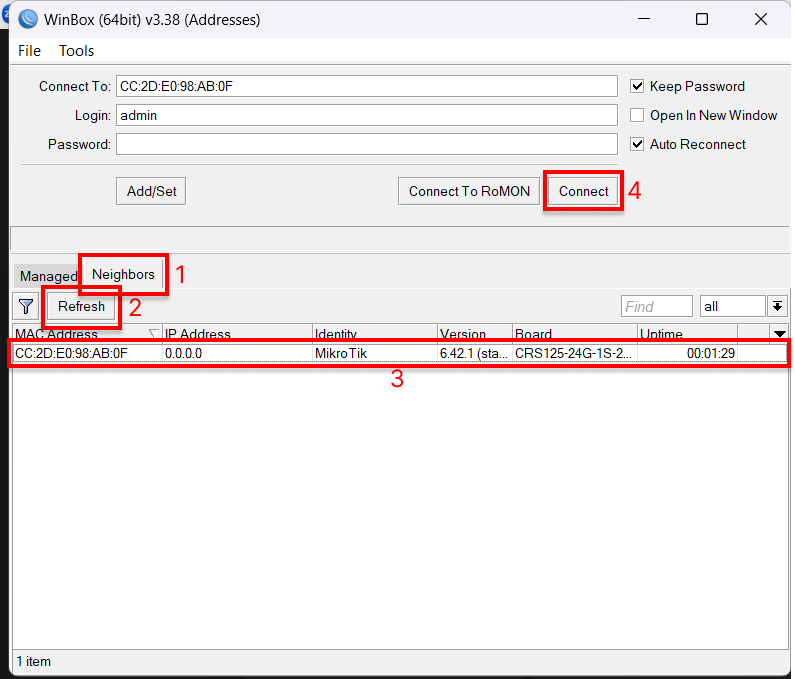
\includegraphics[width=0.5\linewidth]{P3/img/Step 1.png}
			\caption{Step 1}
			\label{fig:Step 1}
		\end{figure}
        \item Jadikan Router menjadi DHCP Client agar bisa mendapat IP address dari Internet ITS. IP > Klik DHCP Client > Tambahkan DHCP Client > Pilih interface yang terhubung dengan Internet (ether6)> Klik Apply > Klik OK.
        \begin{figure}[H]
			\centering
			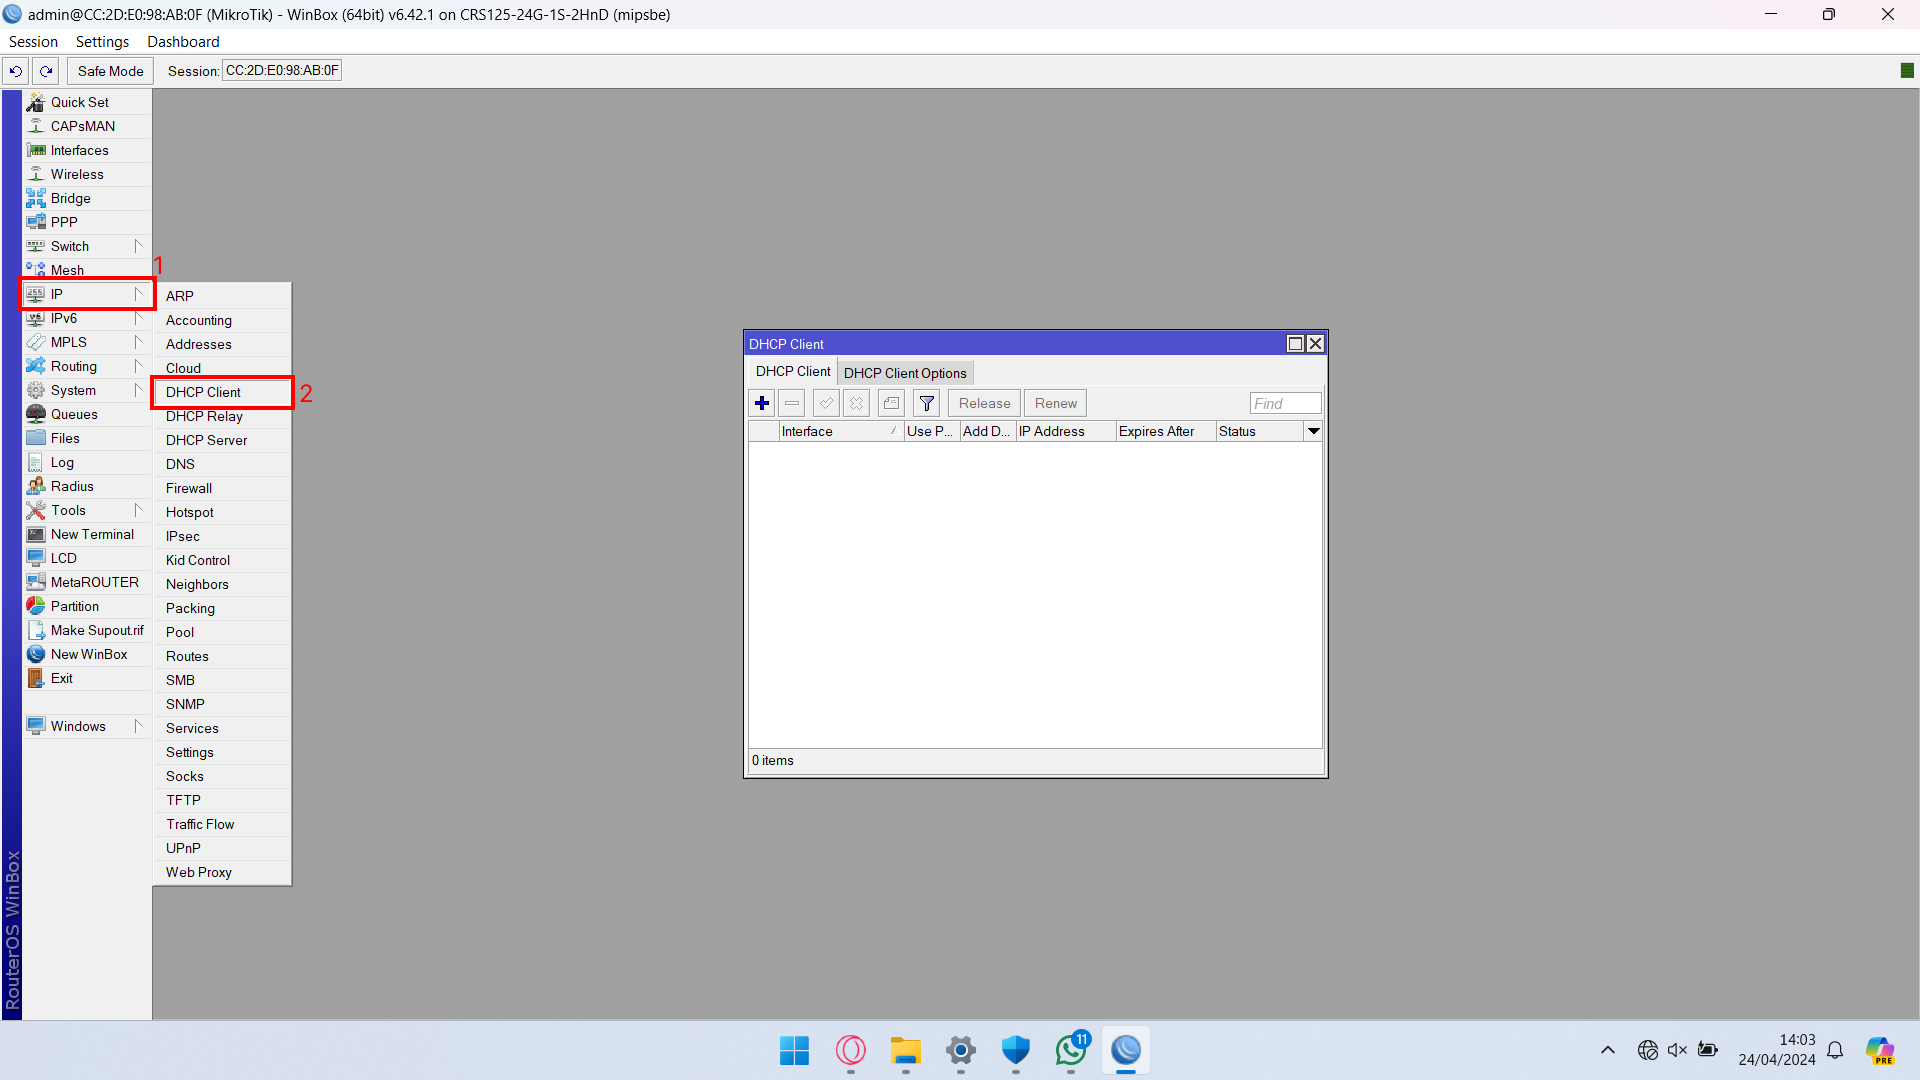
\includegraphics[width=0.8\linewidth]{P3/img/Step 2.1.png}
			\caption{Step 2.1}
			\label{fig:Step 2.1}
		\end{figure}
        \begin{figure}[H]
			\centering
			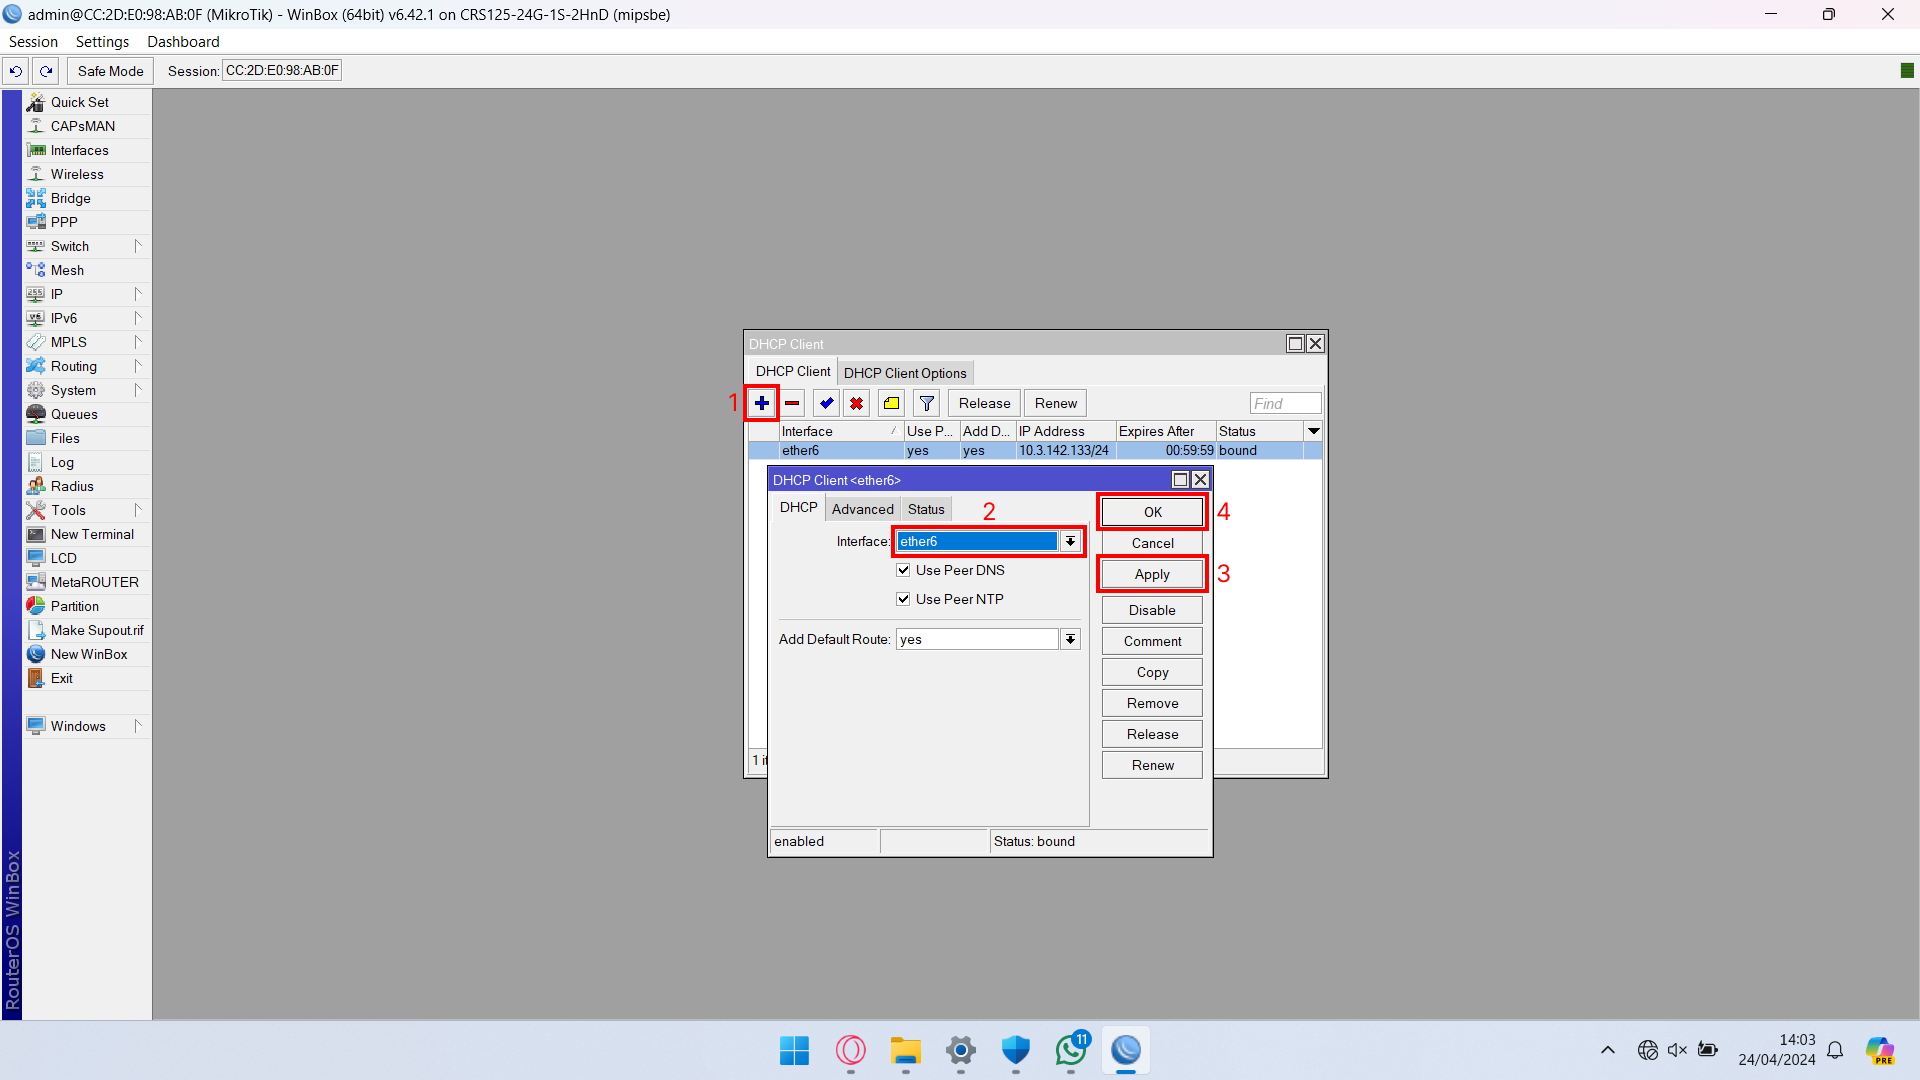
\includegraphics[width=0.8\linewidth]{P3/img/Step 2.2.png}
			\caption{Step 2.2}
			\label{fig:Step 2.2}
		\end{figure}
        \item Buat IP address pada Router yang menghubungkan PC dengan Router. Tambahkan IP address > Isi address > Pilih Interface yang terhubung ke PC (ether2) > Klik Apply > Klik OK.
        \begin{figure}[H]
			\centering
			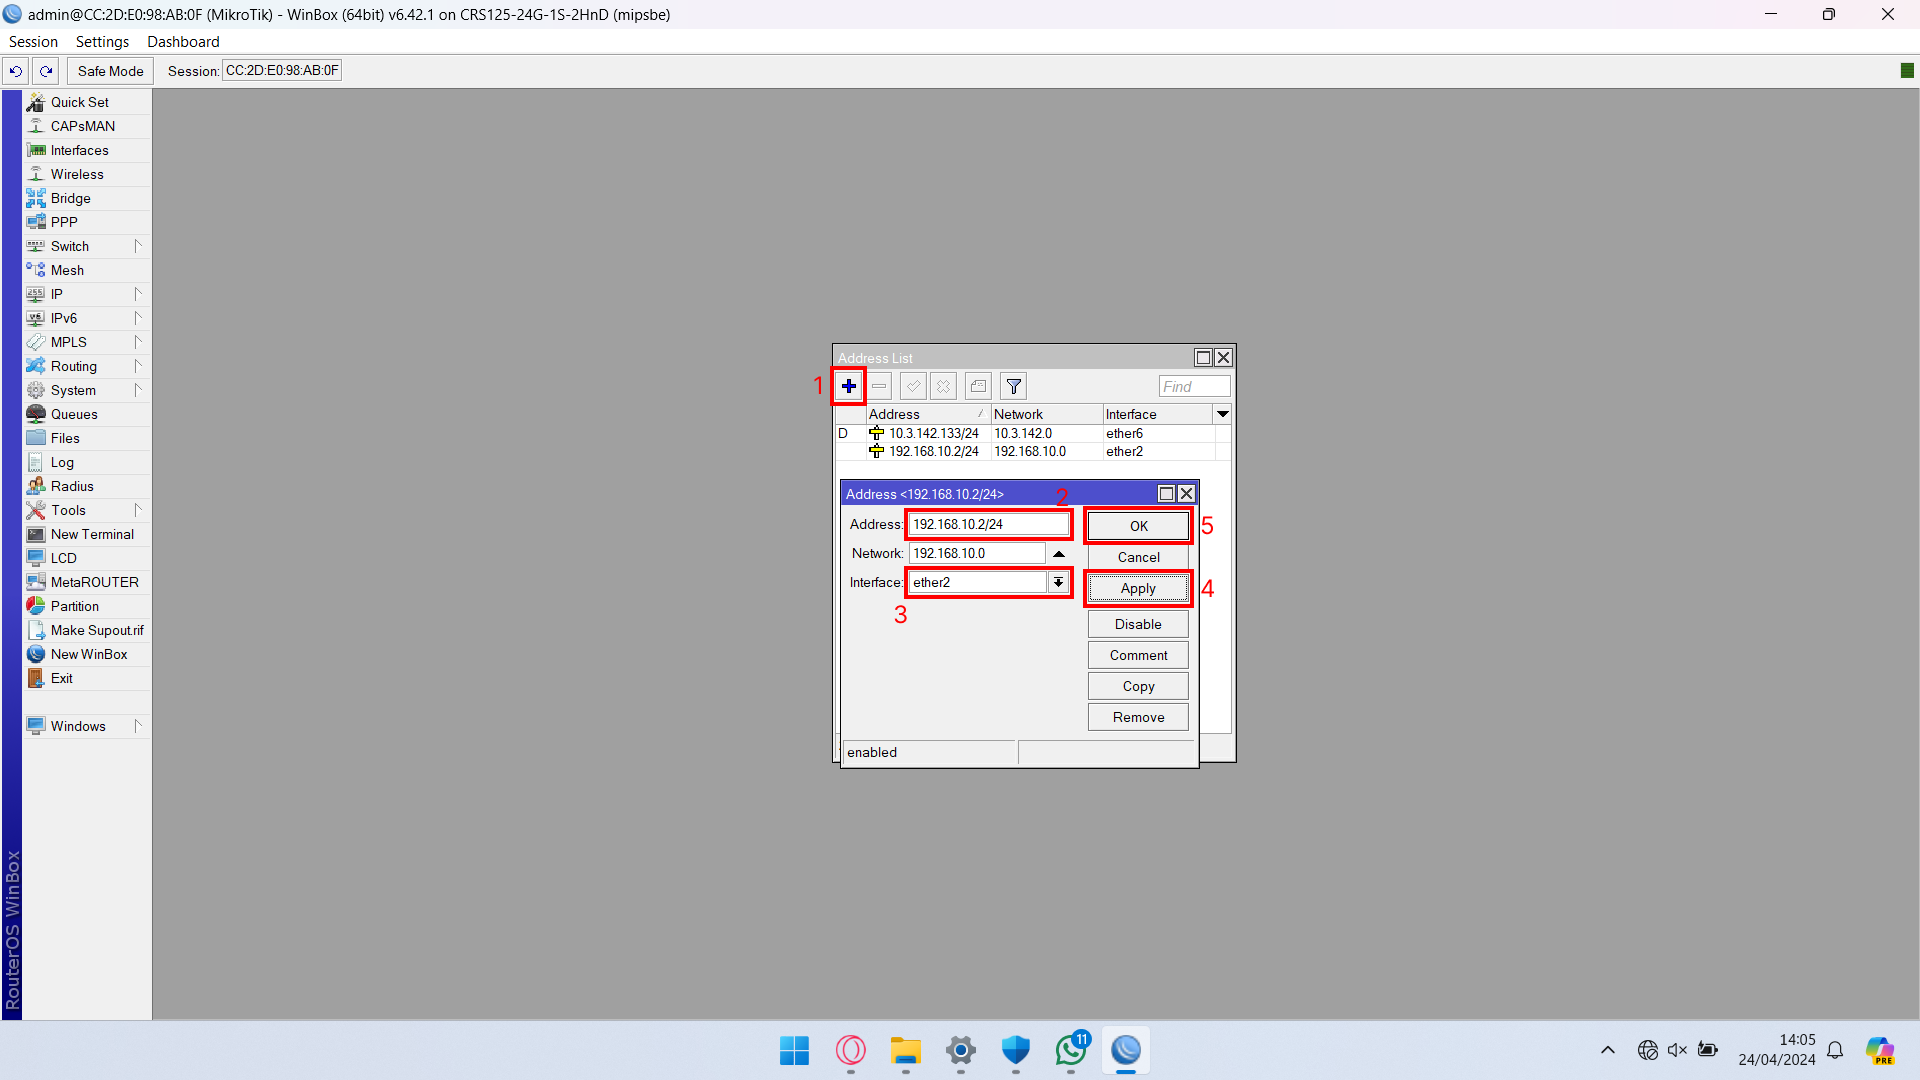
\includegraphics[width=0.8\linewidth]{P3/img/Step 3.png}
			\caption{Step 3}
			\label{fig:Step 3}
		\end{figure}
        \item Jadikan Router menjadi DHCP Server agar bisa memberikan IP address secara DInamis kepada perangkat yang akan terhubung ke Router. IP > Klik DHCP Server
        \begin{figure}[H]
			\centering
			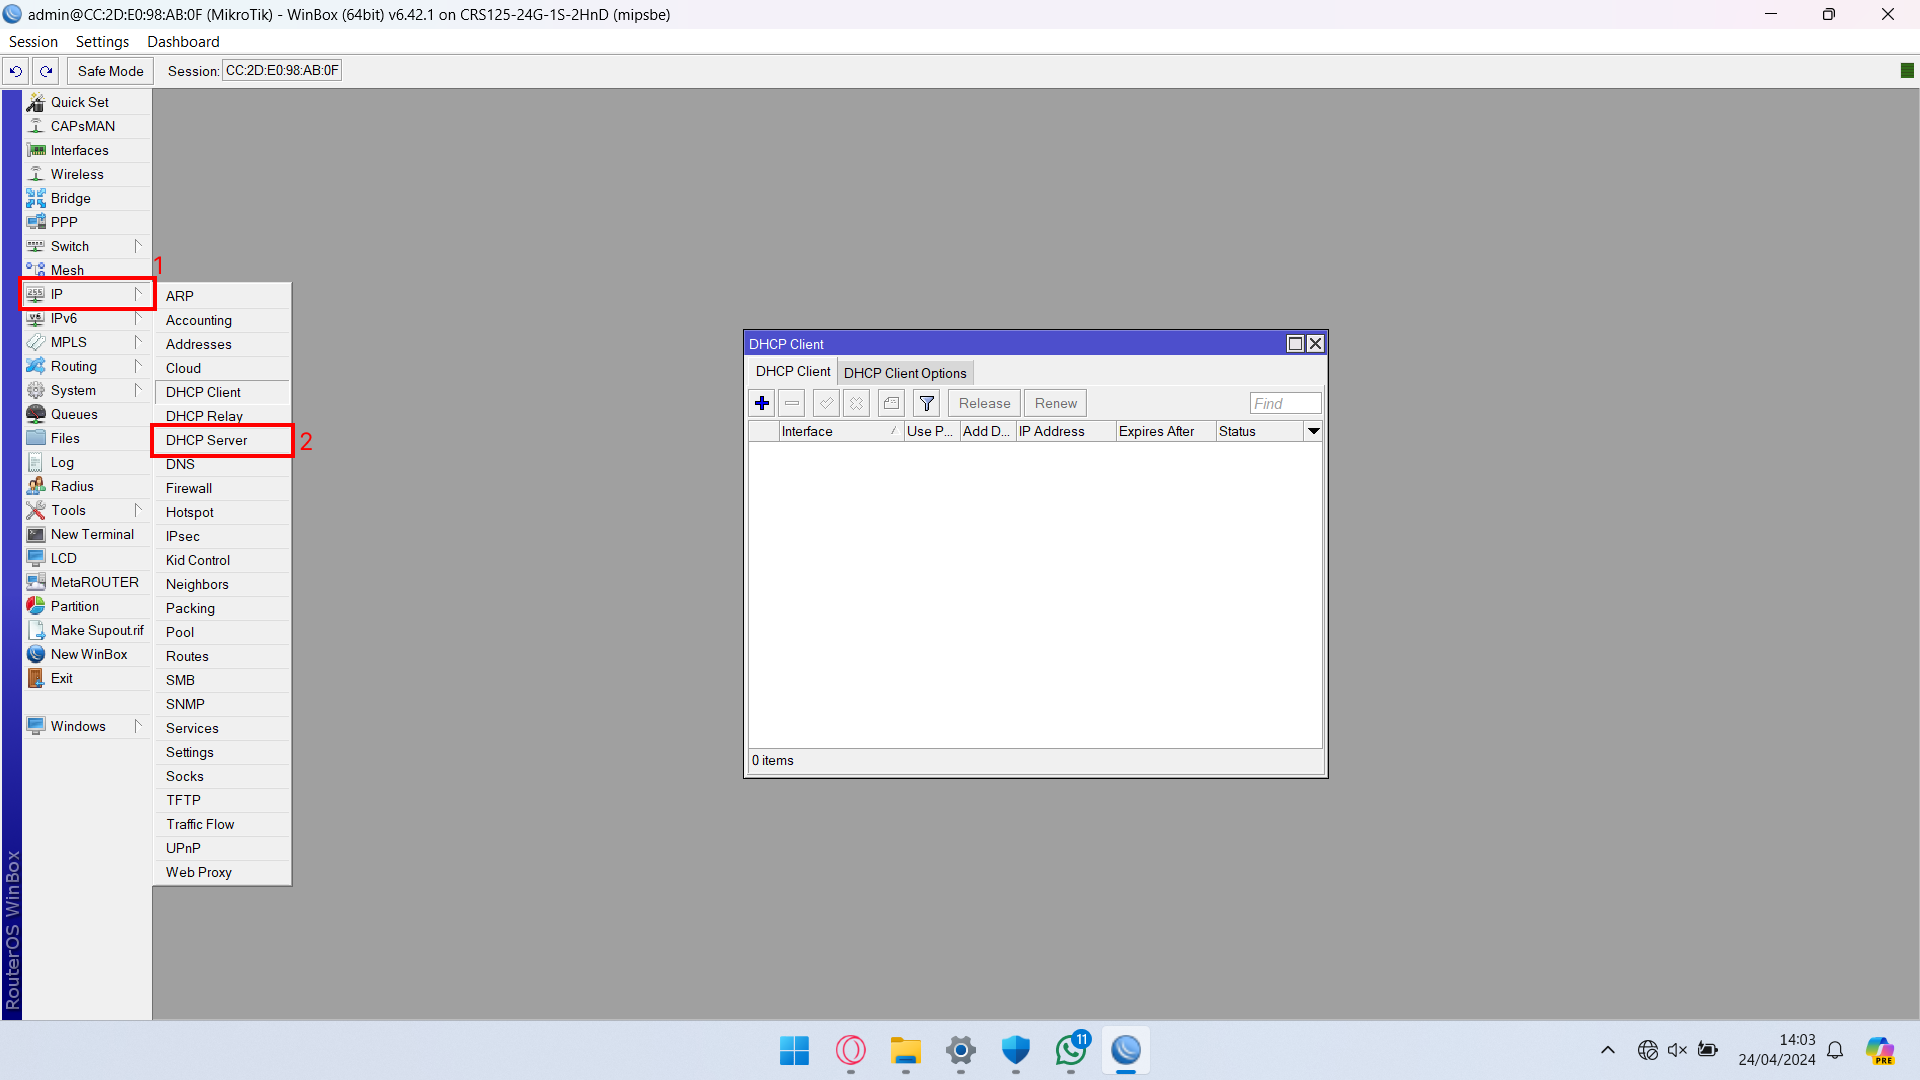
\includegraphics[width=0.8\linewidth]{P3/img/Step 4.png}
			\caption{Step 4}
			\label{fig:Step 4}
		\end{figure}
        \item Untuk menjadikan Router menjadi DHCP Server ada beberapa parameter yang harus di buat. Parameter pertama adalah DHCP Server Interface yang akan menjadi port Output DHCP Server. Klik DHCP Setup > Pilih Interface yang yang akan menjadi Server (ether2).
        \begin{figure}[H]
			\centering
			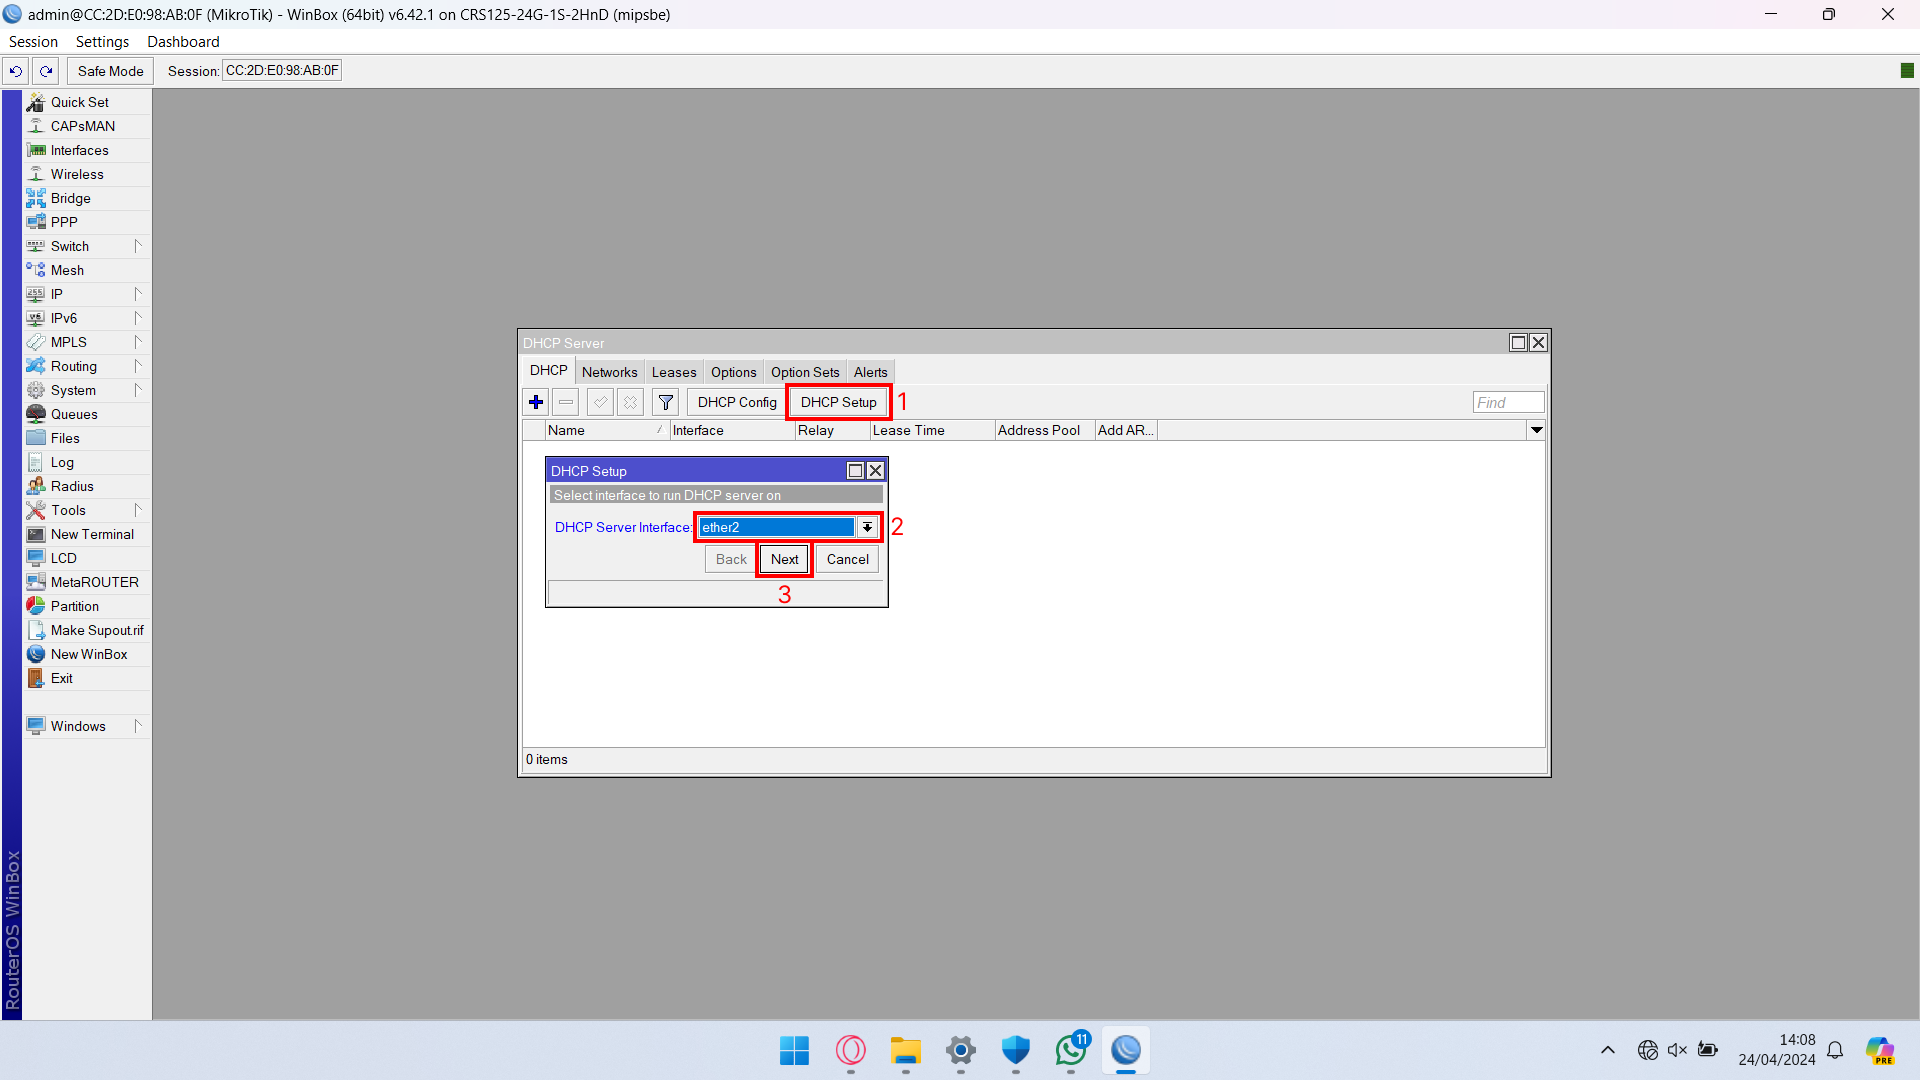
\includegraphics[width=0.8\linewidth]{P3/img/Step 5.png}
			\caption{Step 5}
			\label{fig:Step 5}
		\end{figure}
        \item Parameter kedua adalah DHCP Address Space. Isinya adalah alamat Network yang ingin dibuat. Oleh karena itu alamat IP nya diakhiri dengan angka 0.
        \begin{figure}[H]
			\centering
			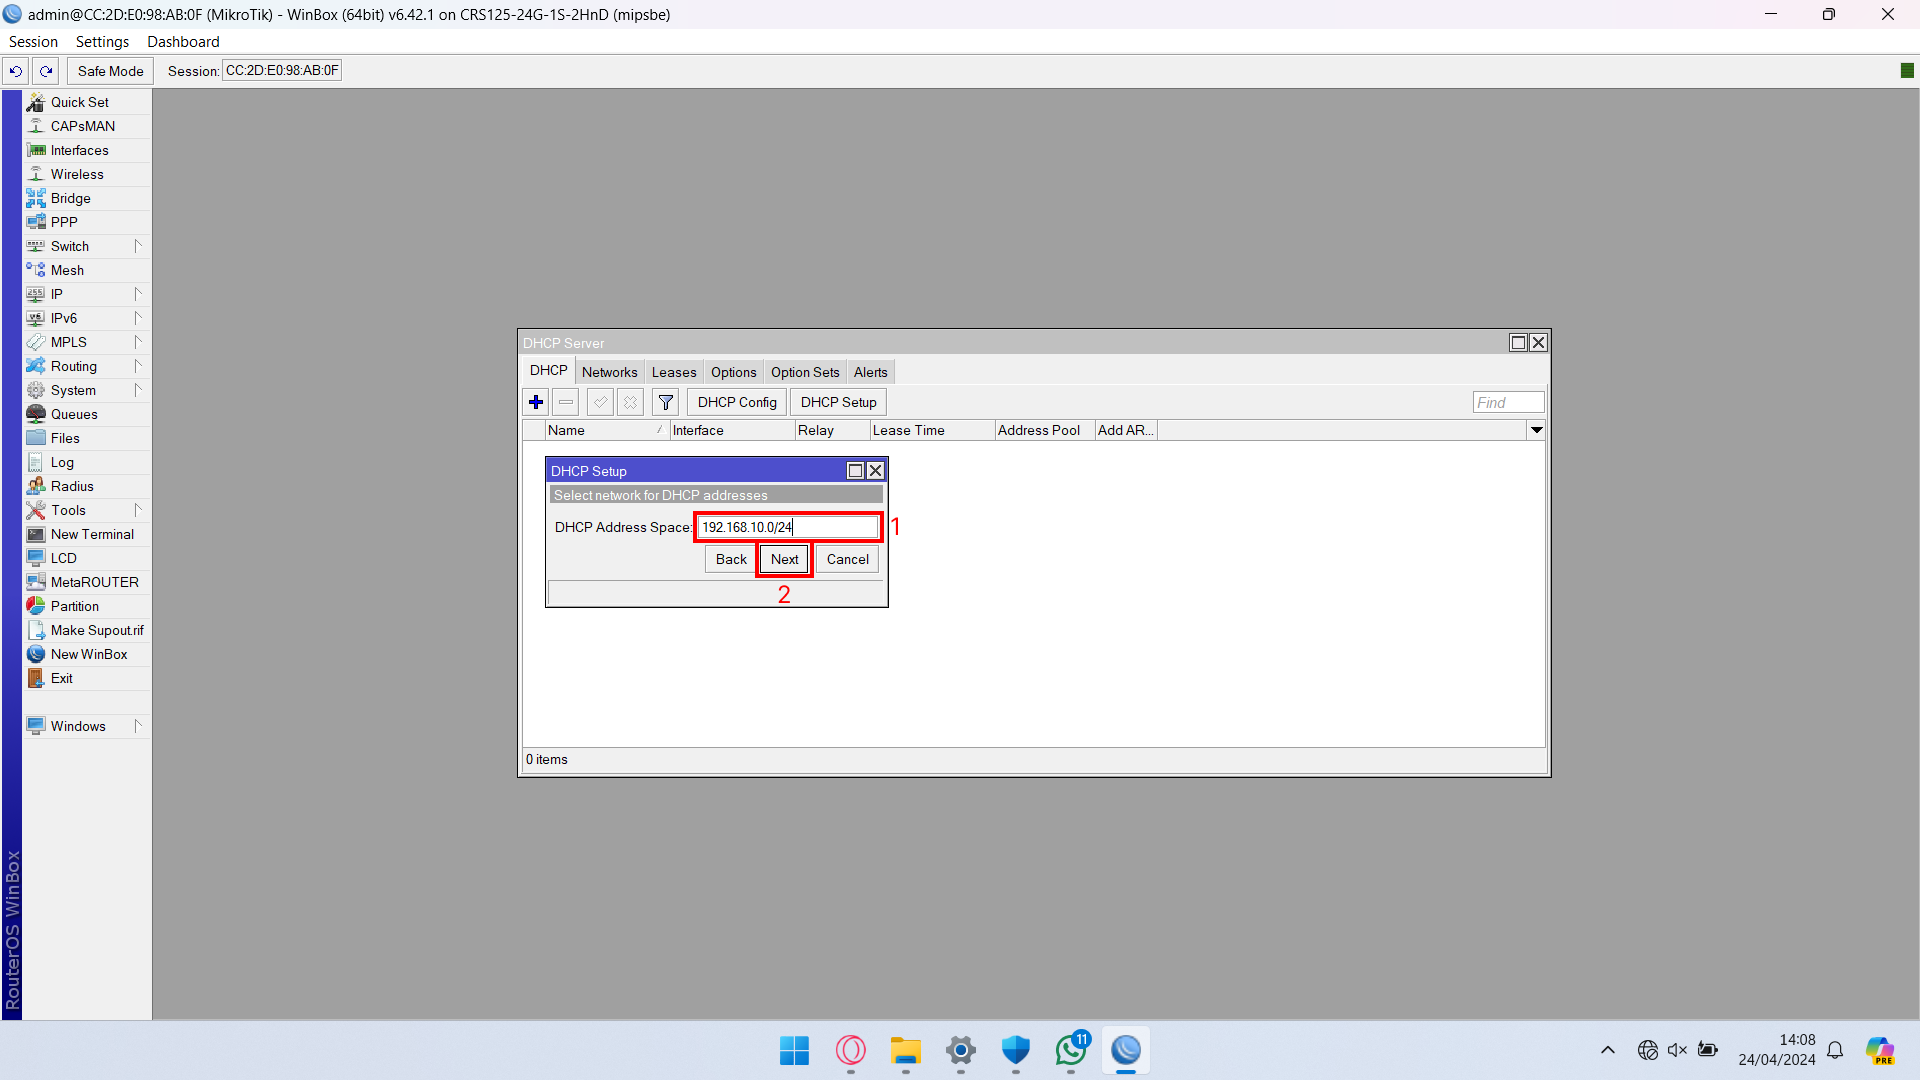
\includegraphics[width=0.8\linewidth]{P3/img/Step 6.png}
			\caption{Step 6}
			\label{fig:Step 6}
		\end{figure}
        \item Parameter ketiga adalah Gateway for DHCP Network. Isinya adalah port pada Router yang akan menghubungkan Router dengan Network address yang sudah ditentukan.
        \begin{figure}[H]
			\centering
			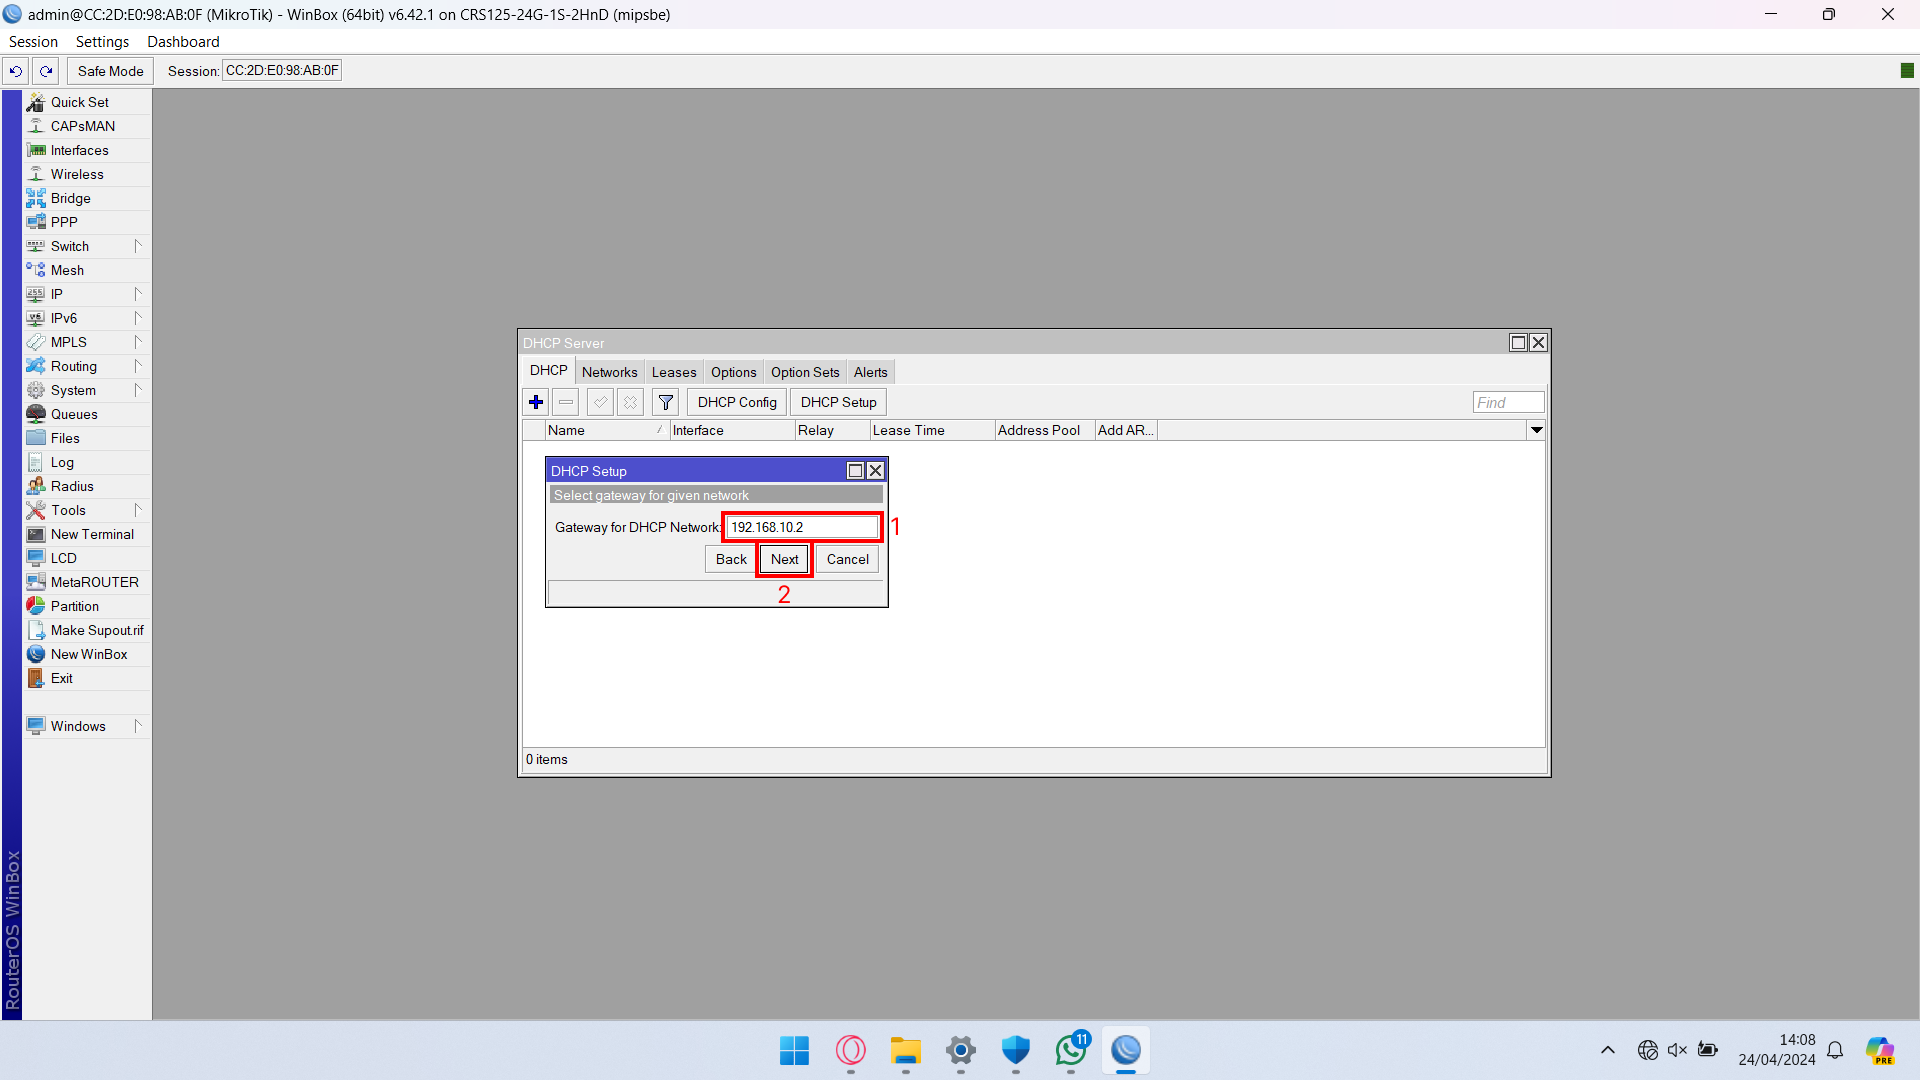
\includegraphics[width=0.8\linewidth]{P3/img/Step 7.png}
			\caption{Step 7}
			\label{fig:Step 7}
		\end{figure}
        \item Parameter keempat adalah Adresses to Give Out. Isinya adalah range IP address yang akan diberikan kepada masing-masing perangkat yang akan terhubung. Pada Modul alamat yang dapat diberikan adalah antara 192.168.10.3 sampai 192.168.10.255.
        \begin{figure}[H]
			\centering
			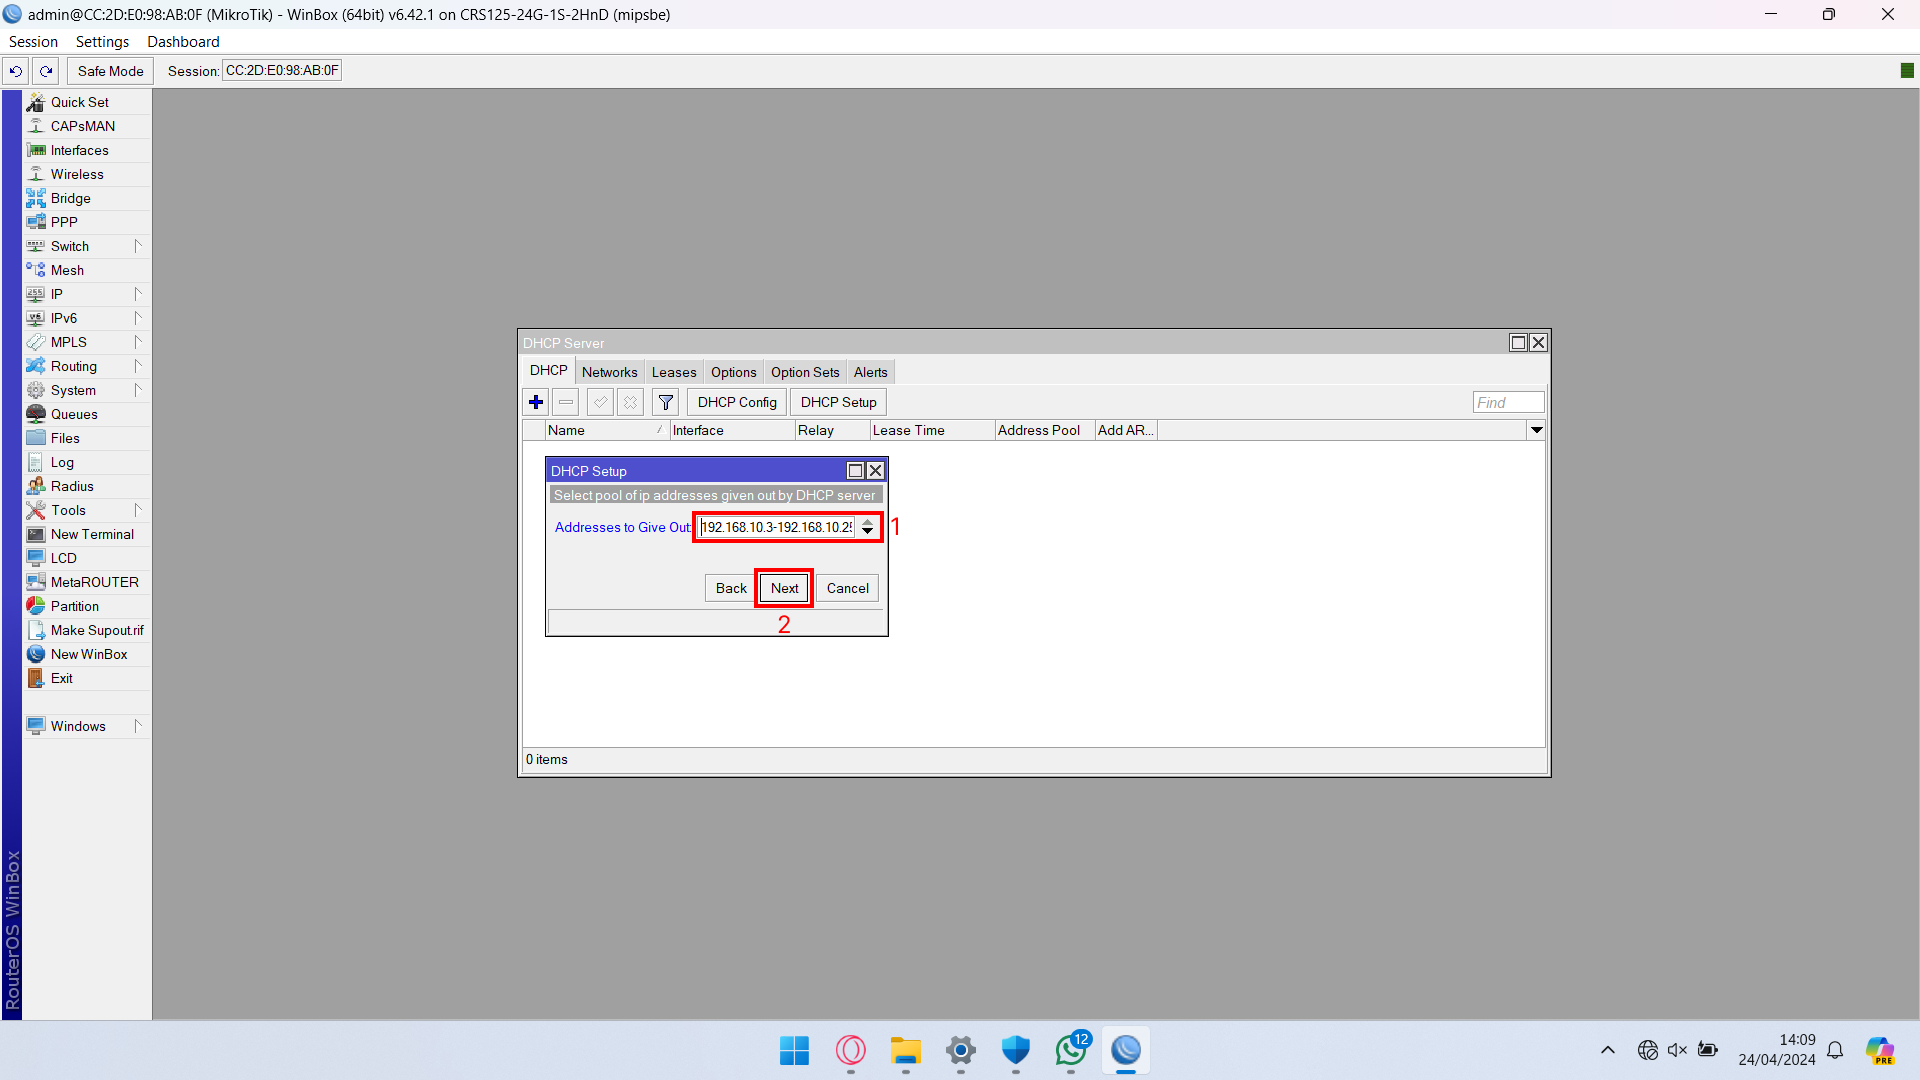
\includegraphics[width=0.8\linewidth]{P3/img/Step 8.png}
			\caption{Step 8}
			\label{fig:Step 8}
		\end{figure}
        \item Parameter kelima adalah DNS Servers. Untuk opsi langsung saja Klik Next.
        \begin{figure}[H]
			\centering
			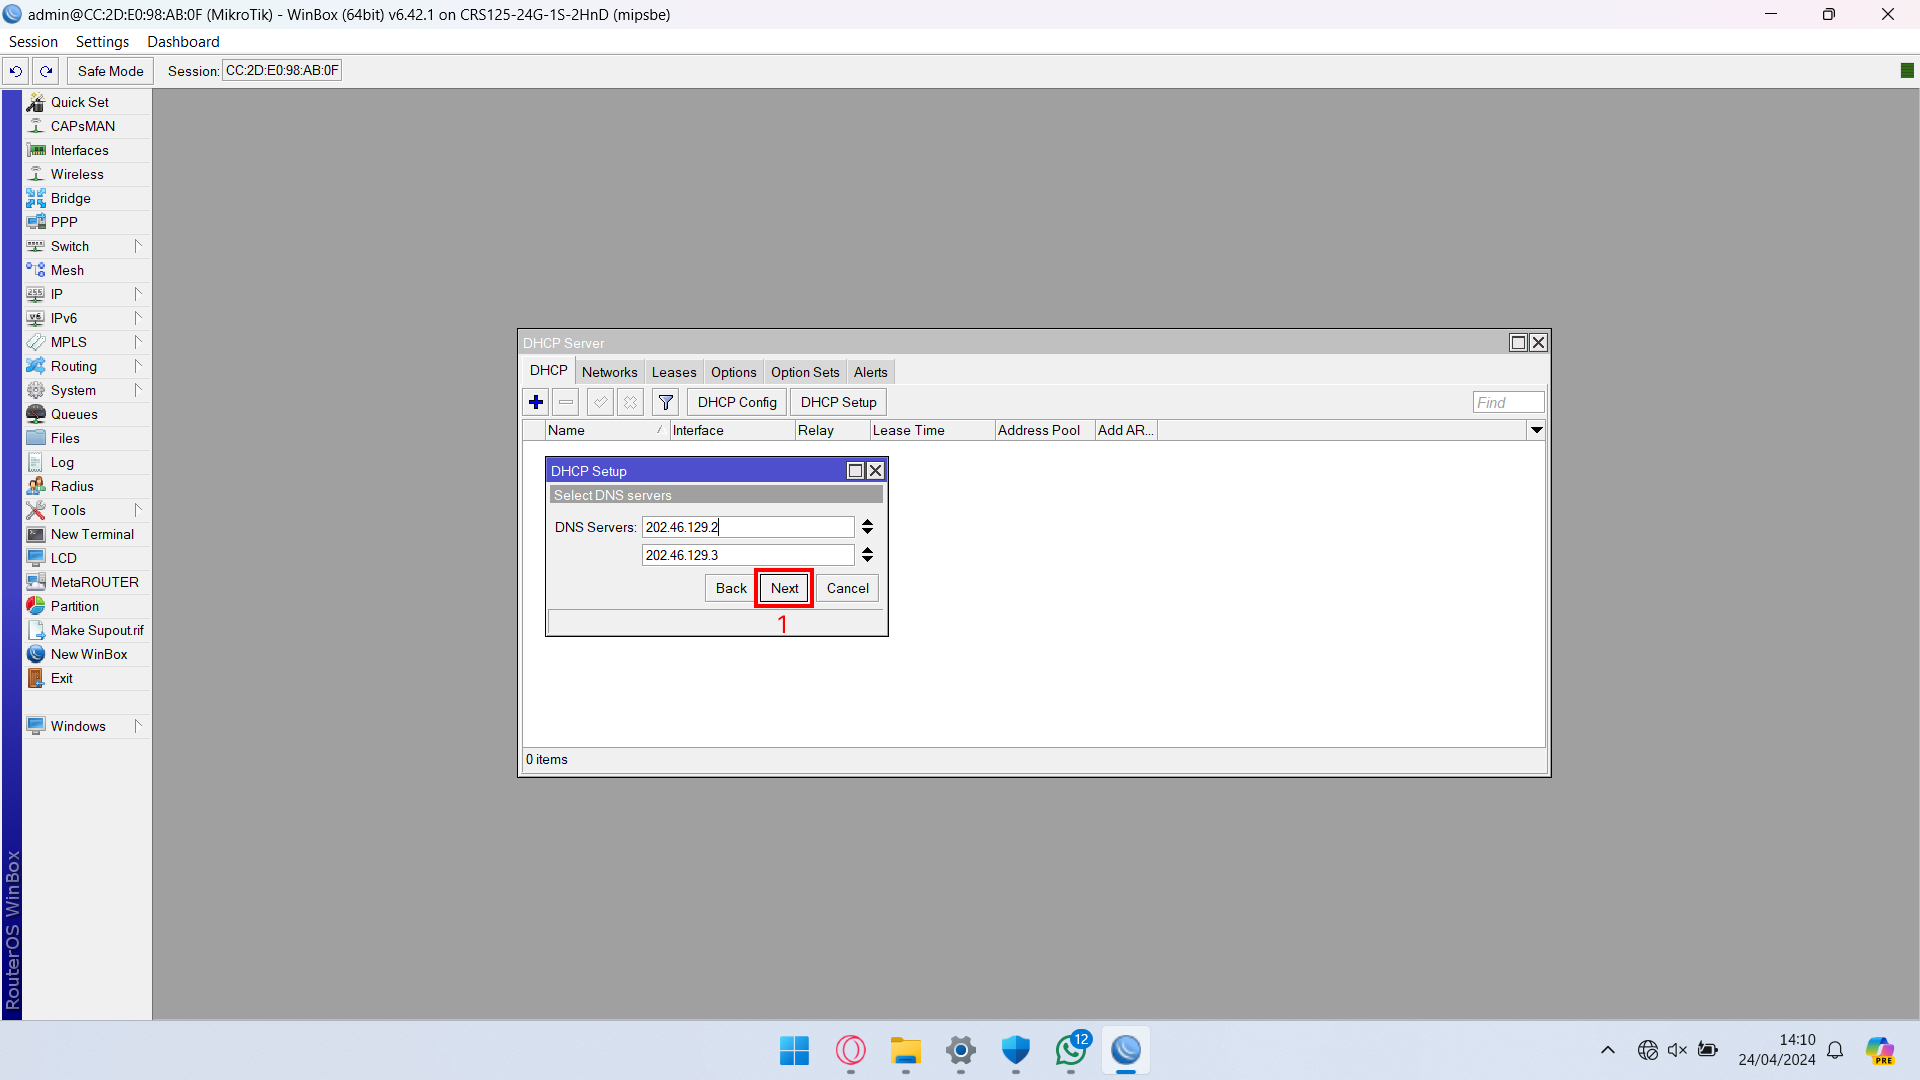
\includegraphics[width=0.8\linewidth]{P3/img/Step 9.png}
			\caption{Step 9}
			\label{fig:Step 9}
		\end{figure}
        \item Parameter keenam adalah Lease Time. Lease Time dipakai untuk membatasi waktu penggunaan IP address yang diberikan oleh Router kepada Devices. Untuk opsi langsung saja Klik Next.
        \begin{figure}[H]
			\centering
			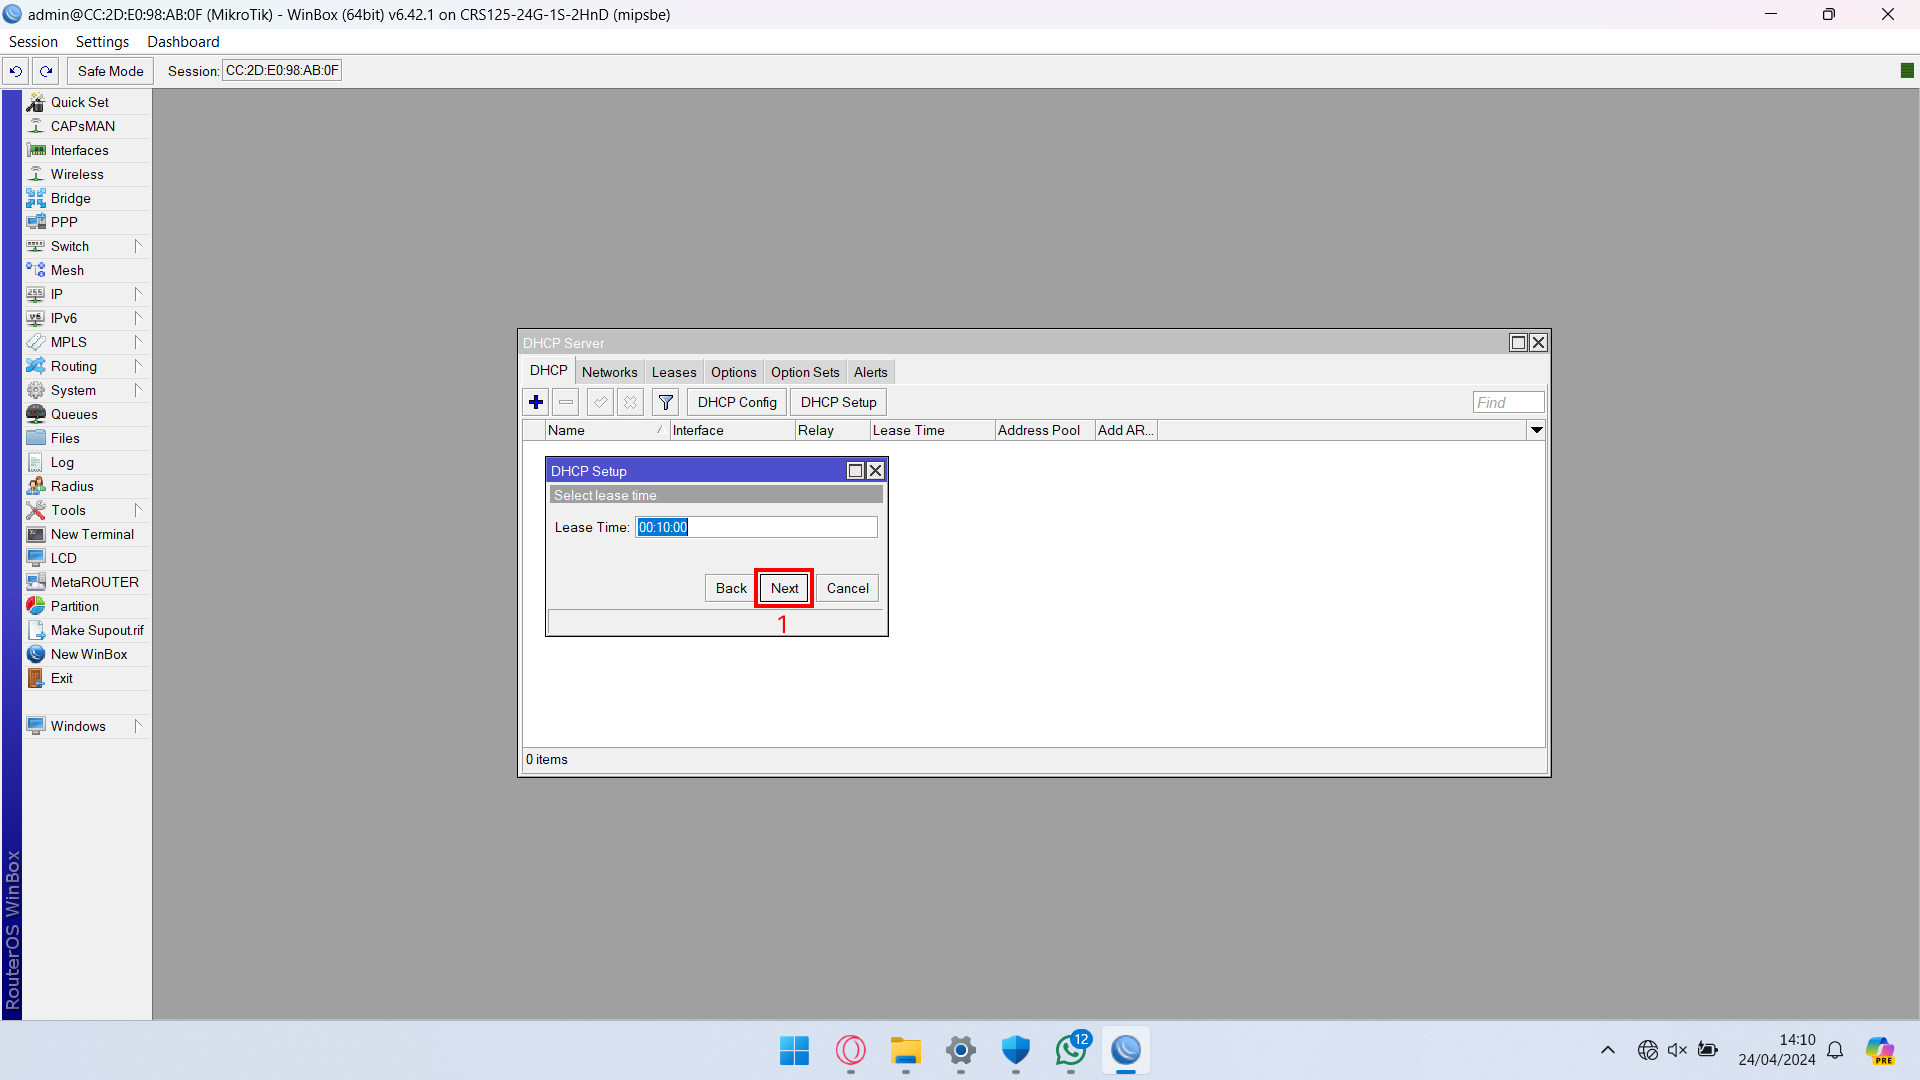
\includegraphics[width=0.8\linewidth]{P3/img/Step 10.png}
			\caption{Step 10}
			\label{fig:Step 10}
		\end{figure}
        \item Pastikan IP Settings untuk koneksi Ethernet pada PC sudah pada Mode Automatic (DHCP).
        \begin{figure}[H]
			\centering
			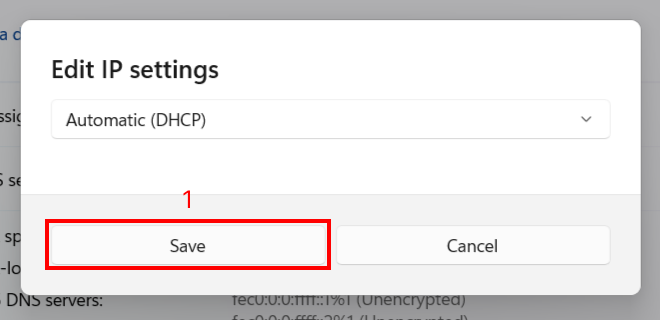
\includegraphics[width=0.8\linewidth]{P3/img/Step 11.png}
			\caption{Step 11}
			\label{fig:Step 11}
		\end{figure}
        \item Agar PC yang berada pada jaringan lokal dapat terhubung ke jaringan publik, dapat digunakan layanan NAT (Network Address Translation) yang akan menerjemahkan IP lokal beserta port perangkat agar dapat terhubung dengan jaringan publik. IP > Klik Firewall.
        \begin{figure}[H]
			\centering
			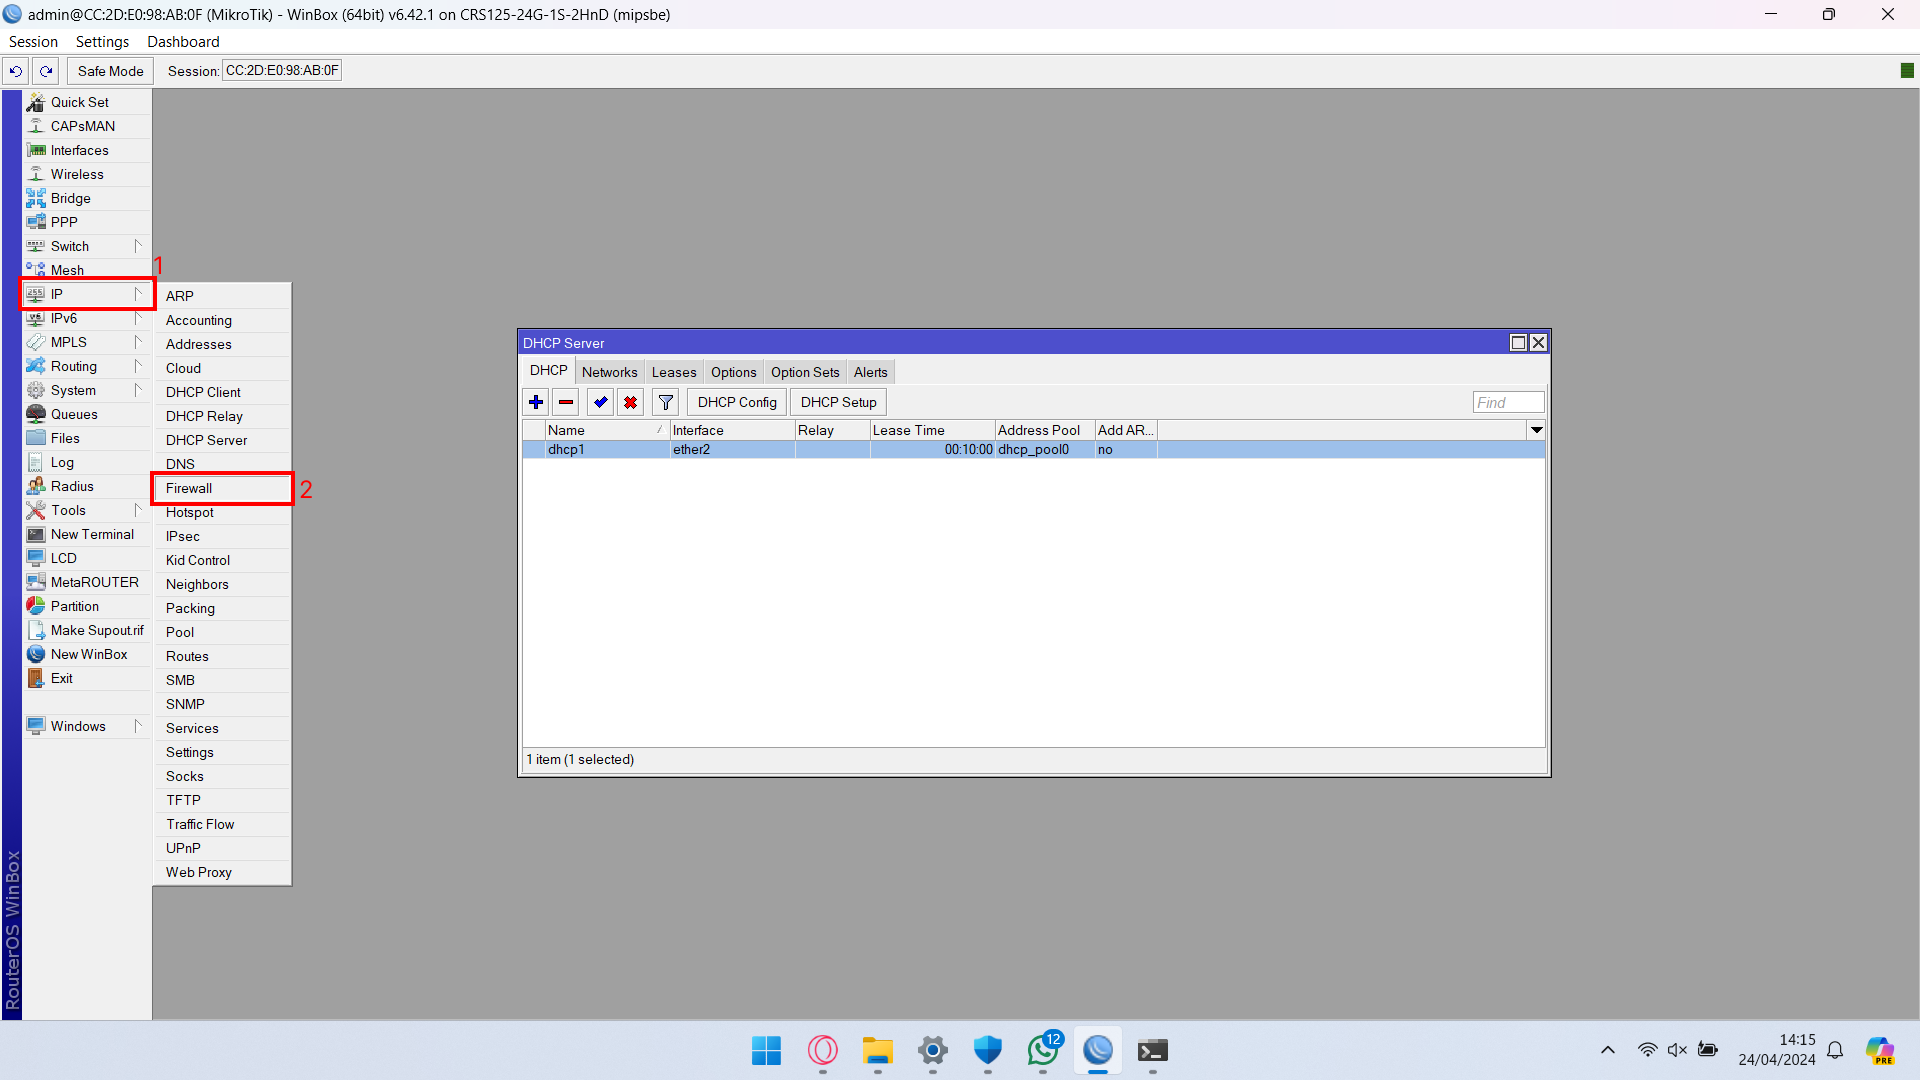
\includegraphics[width=0.8\linewidth]{P3/img/Step 12.png}
			\caption{Step 12}
			\label{fig:Step 12}
		\end{figure}
        \item Buat NAT baru. Klik tab NAT > Tambahkan NAT > Pada Opsi Chain pilih srcnat > Pilih Out Interface yaitu port pada Router yang terhubung dengan Internet(ether6) > Klik Apply. Tambahkan Action pada tab Action. Pada Opsi Action pilih masquerade > Klik Apply > Klik OK.
        \begin{figure}[H]
			\centering
			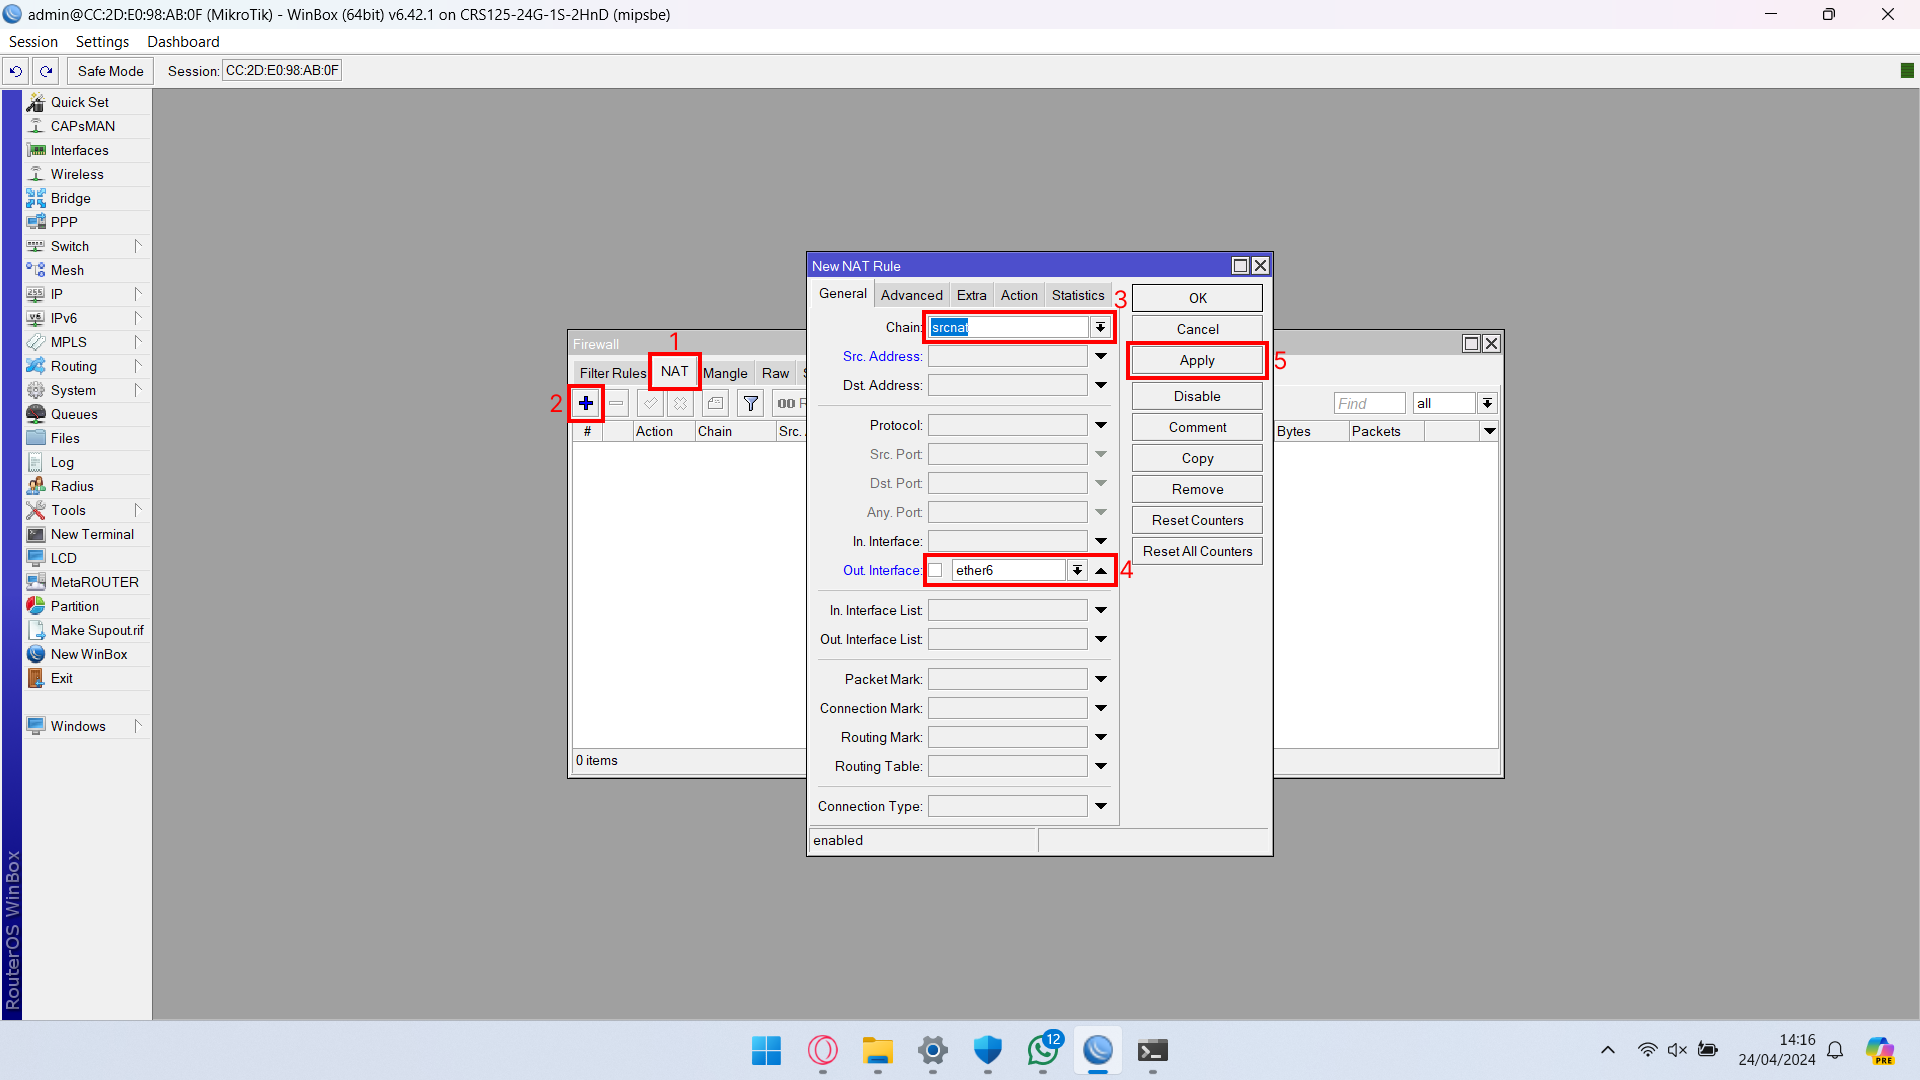
\includegraphics[width=0.8\linewidth]{P3/img/Step 13.png}
			\caption{Step 13.1}
			\label{fig:Step 13.1}
		\end{figure}
        \begin{figure}[H]
			\centering
			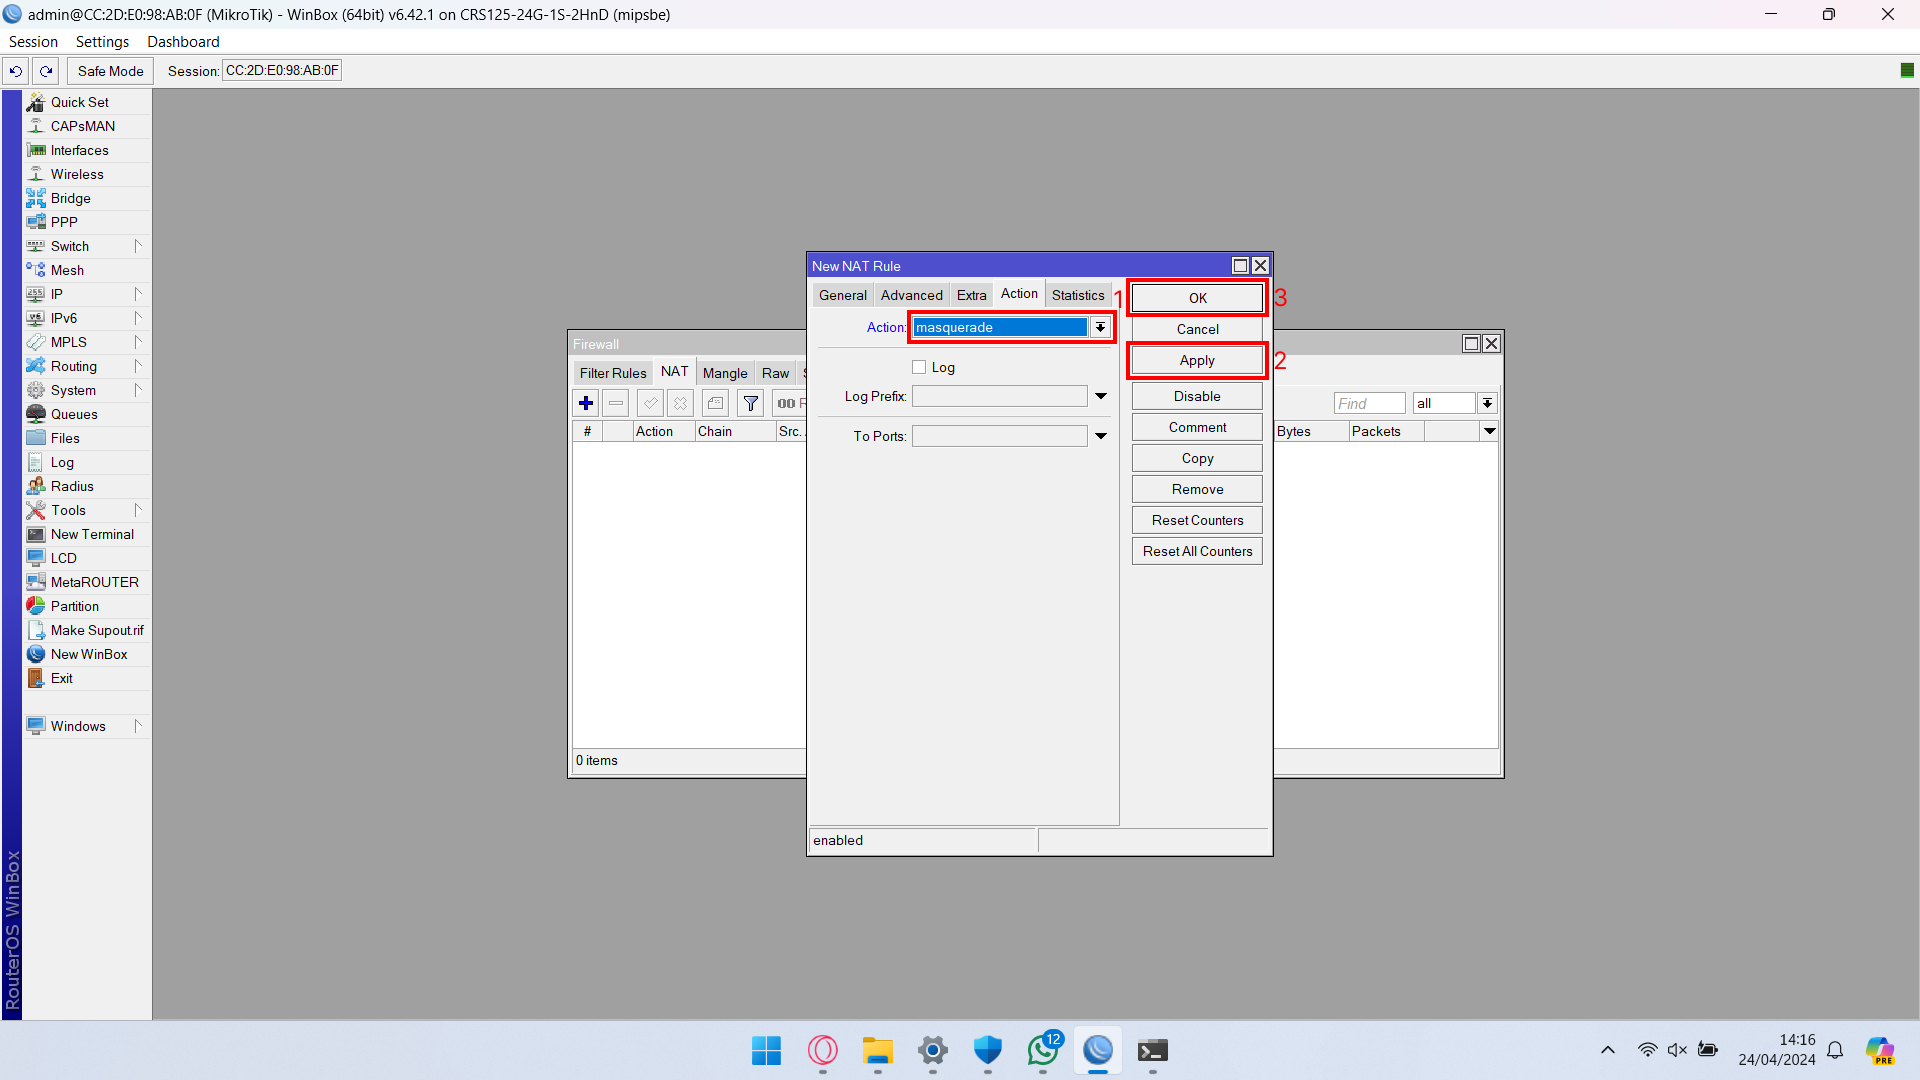
\includegraphics[width=0.8\linewidth]{P3/img/Step 14.png}
			\caption{Step 13.2}
			\label{fig:Step 14.2}
		\end{figure}
        \item Lakukan test ping ke 8.8.8.8 untuk memastikan PC sudah terhubung dengan jaringan luar.
        \begin{figure}[H]
			\centering
			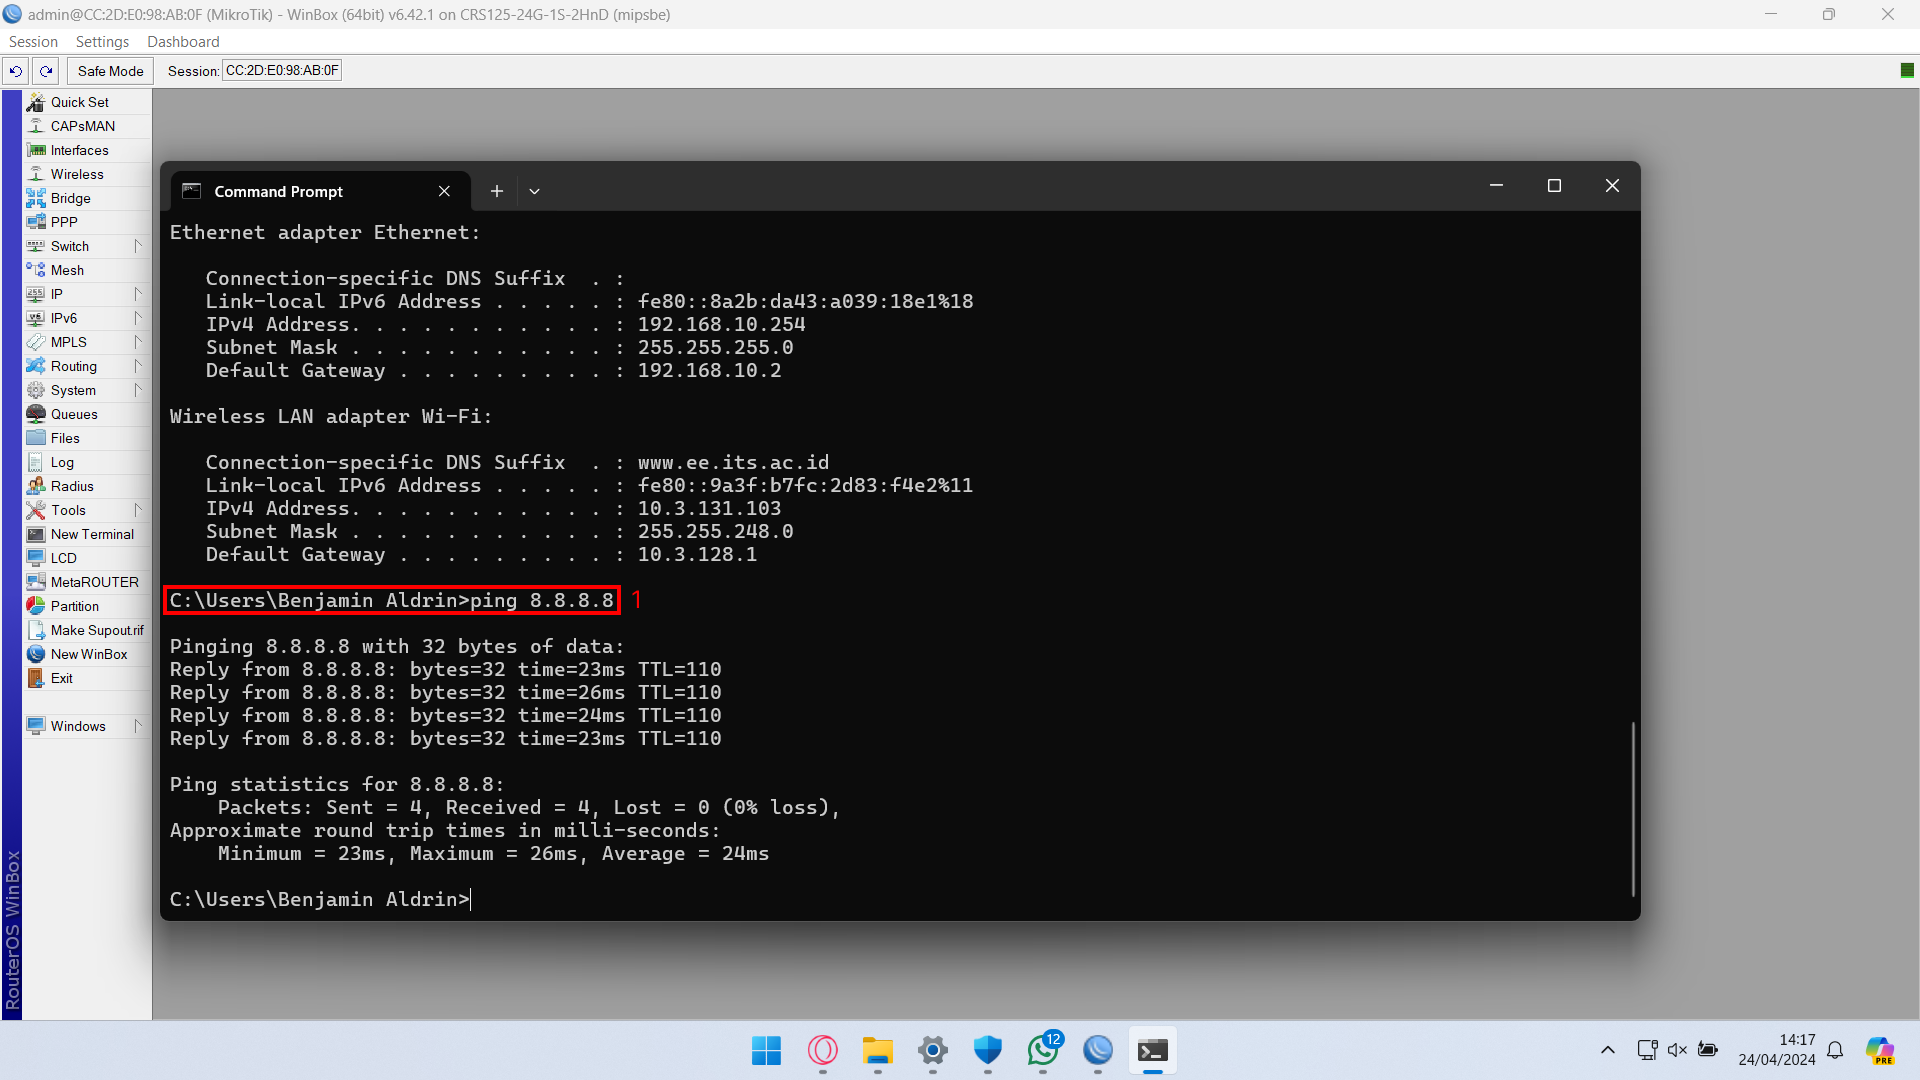
\includegraphics[width=0.8\linewidth]{P3/img/Step 15.png}
			\caption{Step 14}
			\label{fig:Step 14}
		\end{figure}
        \item Lakukan test bandwidth menggunakan SPEEDTEST melalui search engine PC.
        \begin{figure}[H]
			\centering
			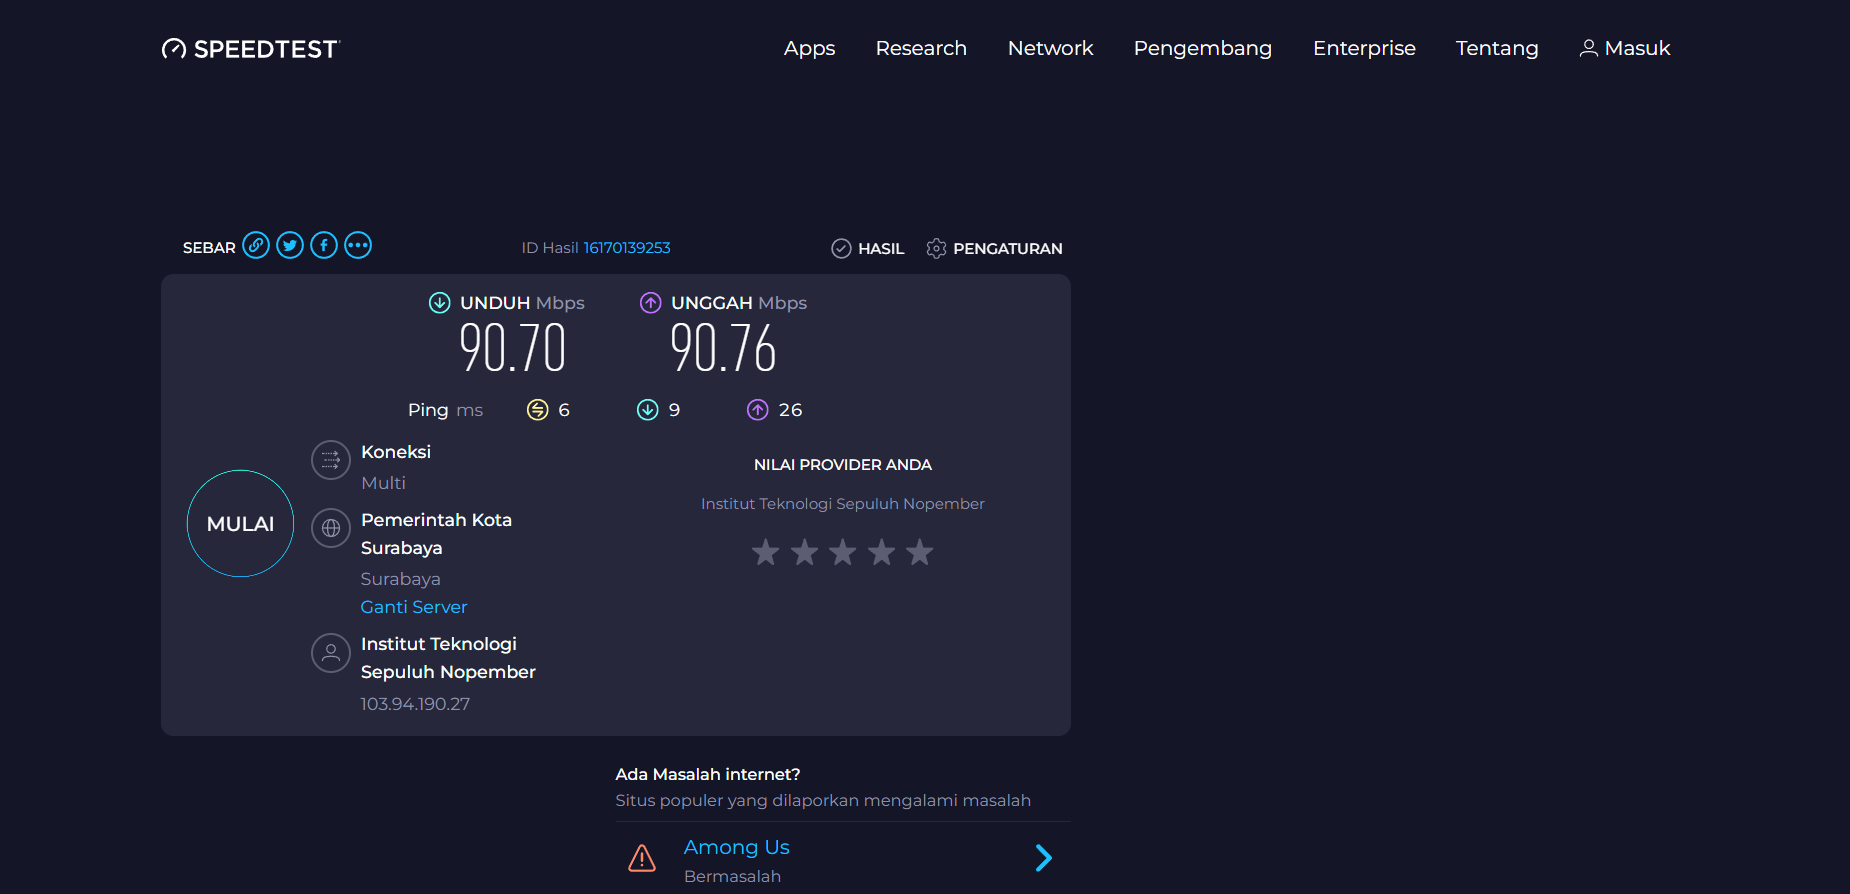
\includegraphics[width=0.8\linewidth]{P3/img/Step 16.png}
			\caption{Step 15}
			\label{fig:Step 15}
		\end{figure}
        \item Lakukan pembatasan bandwidht menggunakan Queues. Klik Queues,  Klik Queues > Tambahkan Queue List > Isi Nama perangkat yang ingin dibatasi bandwidthnya > Isi target dengan IP address PC (dapat dilihat melalui ipconfig) > Batasi Target Uploadnya menjadi 1M > Batasi Target Downloadnya menjadi 1M > Klik Apply > Klik OK.
        \begin{figure}[H]
			\centering
			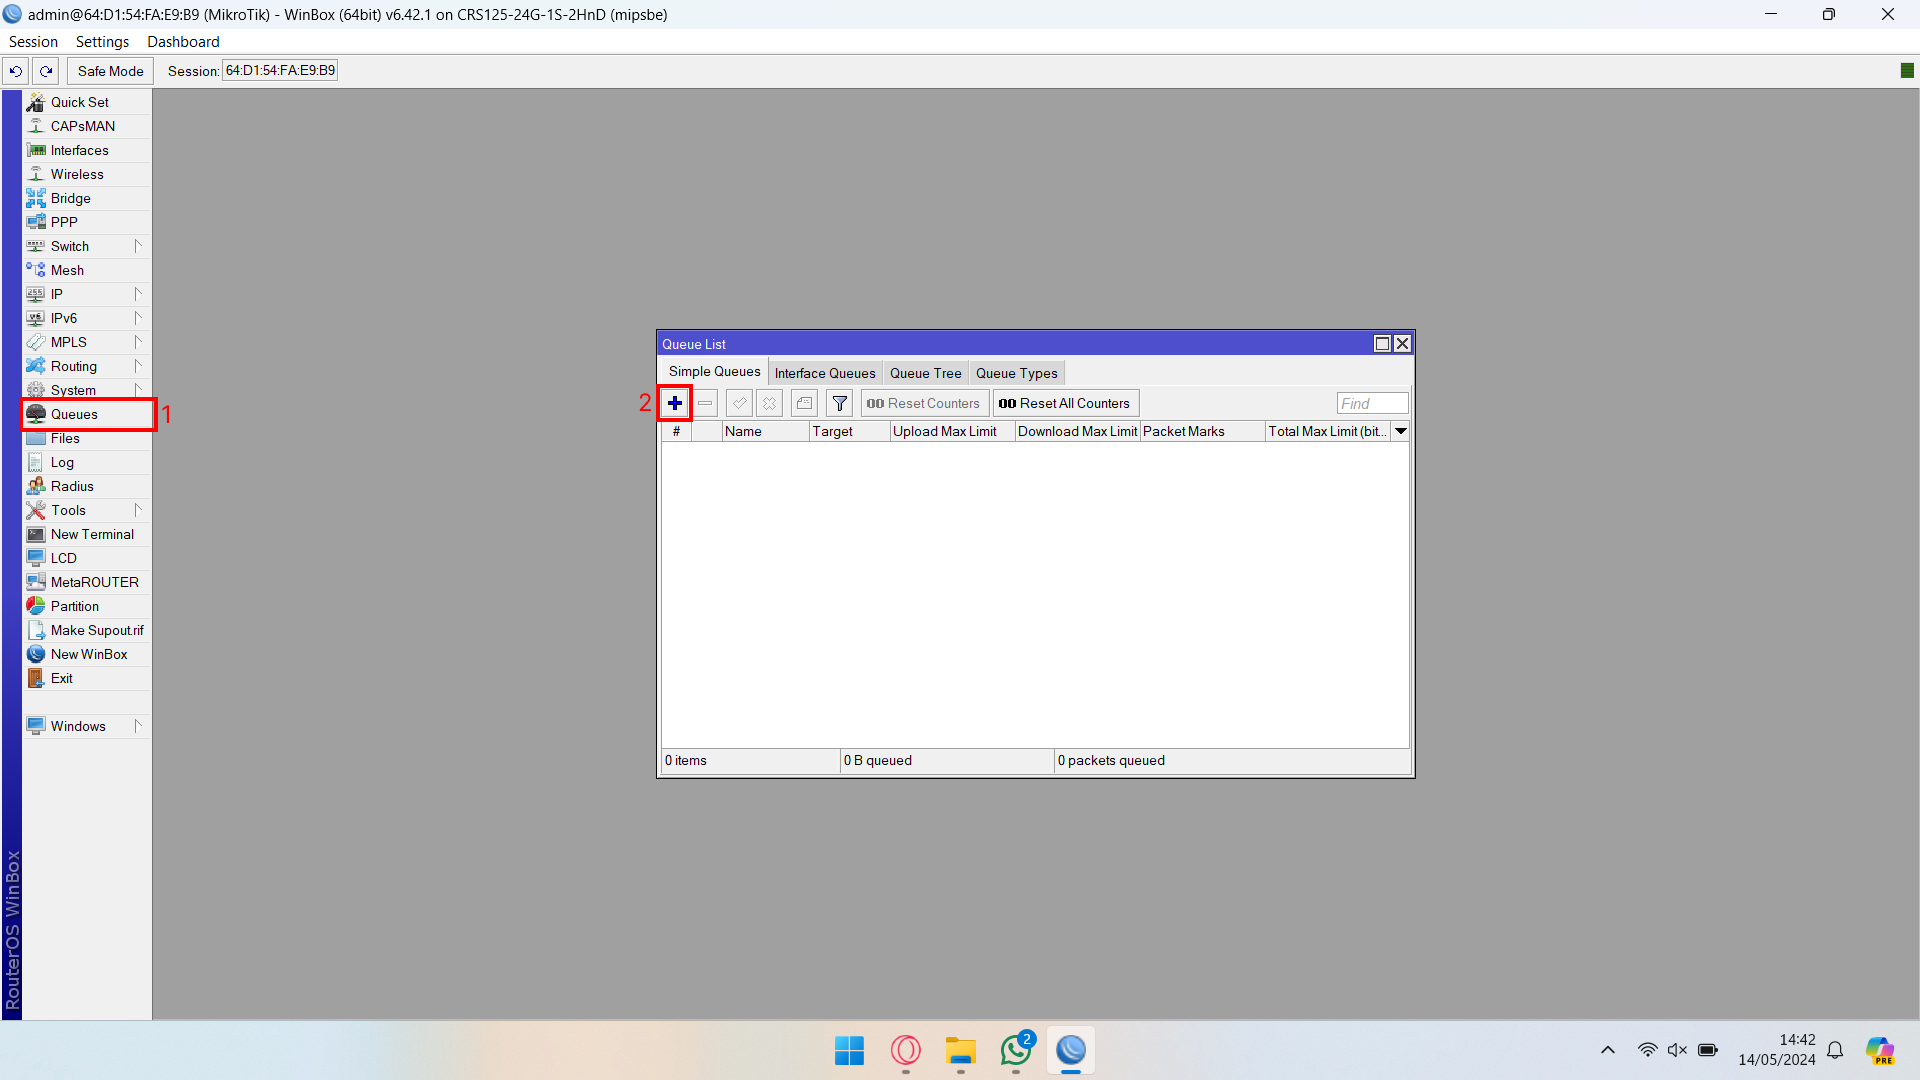
\includegraphics[width=0.8\linewidth]{P3/img/Step 17.png}
			\caption{Step 16.1}
			\label{fig:Step 16.1}
		\end{figure}
        \begin{figure}[H]
			\centering
			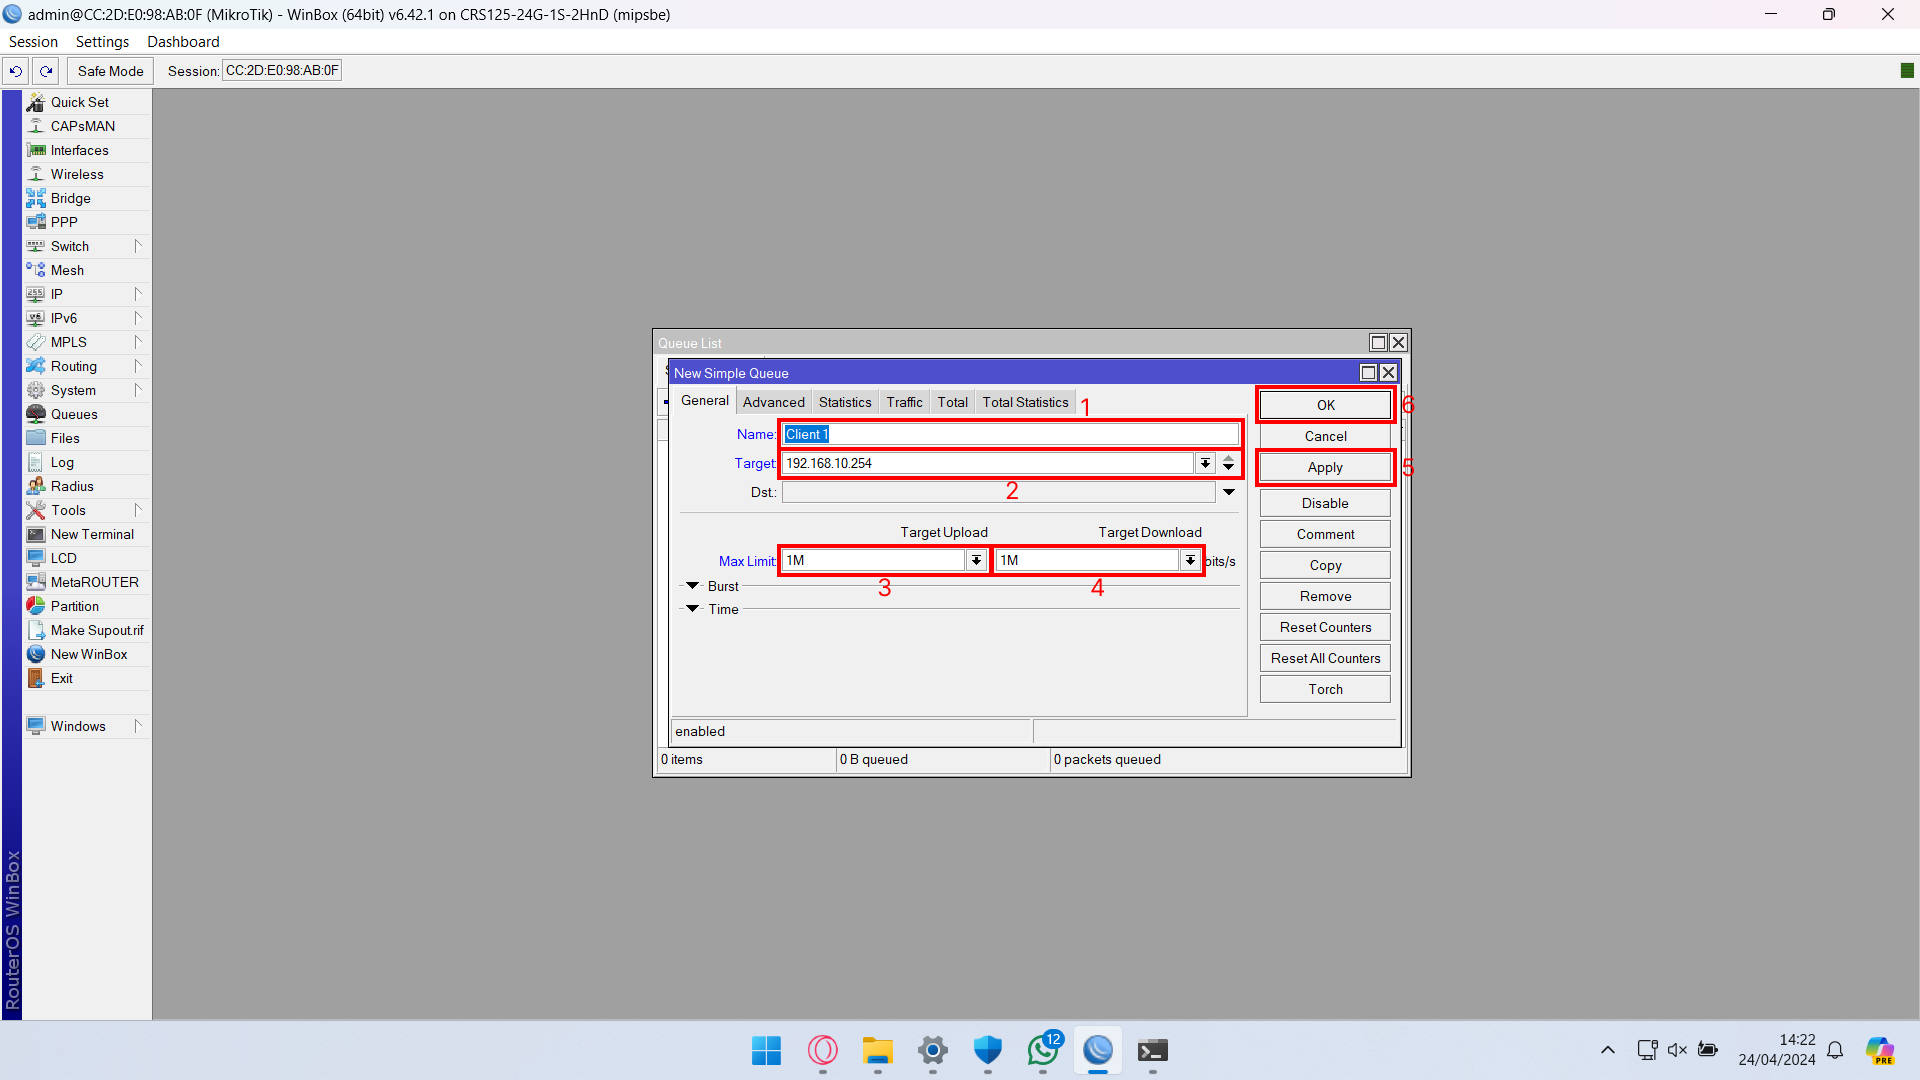
\includegraphics[width=0.8\linewidth]{P3/img/Step 18.png}
			\caption{Step 16.2}
			\label{fig:Step 16.2}
		\end{figure}
        \item Lakukan test bandwidth kembali menggunakan SPEEDTEST melalui search engine PC.
        \begin{figure}[H]
			\centering
			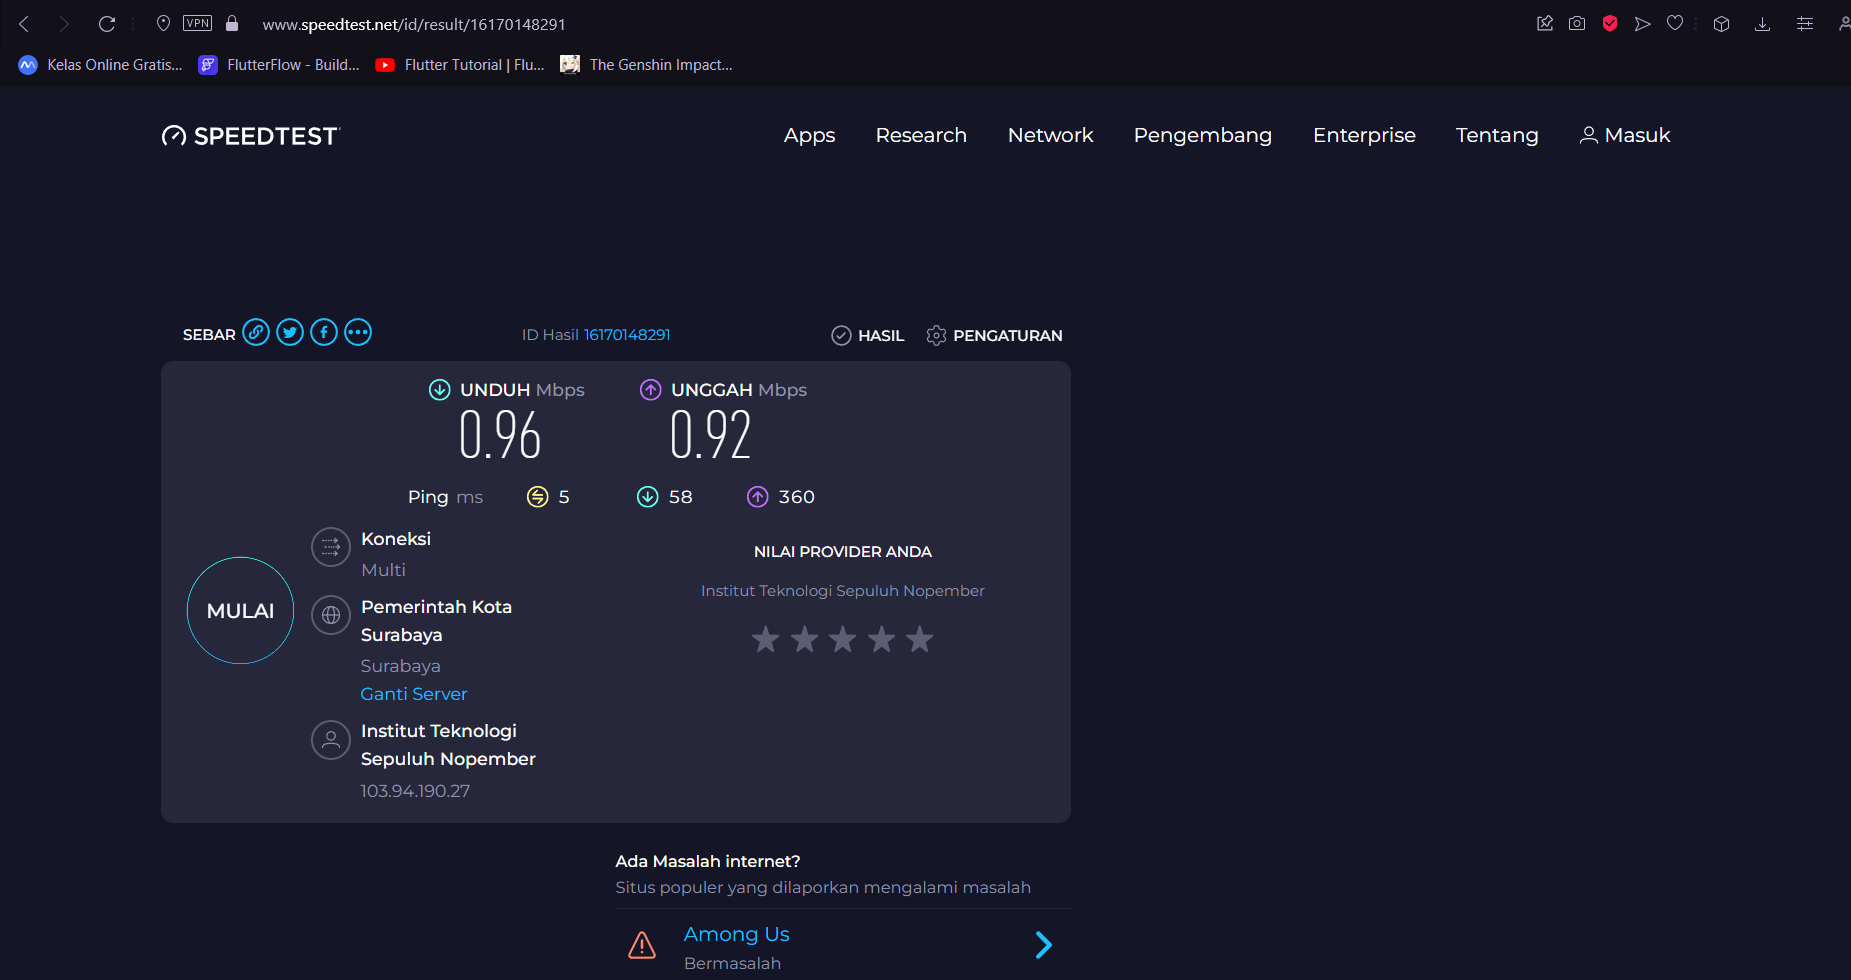
\includegraphics[width=0.8\linewidth]{P3/img/Step 19.png}
			\caption{Step 17}
			\label{fig:Step 17}
		\end{figure}
    \end{enumerate}
\end{center}

%===========================================================%
\section{Hasil yang didapat}
Memahami dan mengkonfigurasi routing dinamis RIP dengan tepat.

%===========================================================%
\section{Kesimpulan}
Dalam mengkonfigurasi routing RIP, diperlukan pemahaman dasar mengenai setting IP Address dan Subnetting, dan juga diperlukan ketelitian dan fokus agar berhasil
